% 独自のコマンド

% ■ アブストラクト
%	\begin{jabstract} 〜 \end{jabstract}	:日本語のアブストラクト
%	\begin{eabstract} 〜 \end{eabstract}	:英語のアブストラクト

% ■ 謝辞
%	\begin{acknowledgment} 〜 \end{acknowledgment}

% ■ 文献リスト
%	\begin{bib}[100] 〜 \end{bib}


\newif\ifjapanese

\japanesetrue	% 論文全体を日本語で書く(英語で書くならコメントアウト)

\ifjapanese
	\documentclass[11pt]{jreport}
	\renewcommand{\bibname}{参考文献}
	\newcommand{\acknowledgmentname}{謝辞}
\else
	\documentclass[11pt]{report}
	\newcommand{\acknowledgmentname}{Acknowledgment}
\fi
\usepackage[top=30truemm,bottom=30truemm,left=25truemm,right=25truemm]{geometry}
\usepackage{ascmac}
\usepackage{graphicx}
\usepackage{multirow}
\usepackage{ylab_thesis}
\DeclareFontShape{JY1}{mc}{m}{it}{<5> <6> <7> <8> <9> <10> sgen*min
    <10.95><12><14.4><17.28><20.74><24.88> min10 <-> min10}{}
\DeclareFontShape{JT1}{mc}{m}{it}{<5> <6> <7> <8> <9> <10> sgen*tmin
    <10.95><12><14.4><17.28><20.74><24.88> tmin10 <-> tmin10}{}
\usepackage{times}
\usepackage[stable]{footmisc}
\usepackage{otf}
\usepackage{epsf}

%\bindermode	% バインダ用余白設定

% 日本語情報(必要なら)
\jclass	{卒業論文}							% 論文種別
\jtitle		{睡眠中の夢は外的刺激により操作できるのか?\\スマートフォンアプリDreamtravelerの\\提案と検証}			% タイトル。改行する場合は\\を入れる
%明晰夢を実現することで拡張現実を実現することは可能なのか?
\juniv		{慶應義塾大学}						% 大学名
\jfaculty	{環境情報学部環境情報学科}				% 学部、学科
\jauthor	{樋山 理紗}						% 著者 \CID{7808}でも同字が出る
\jnumber	{71247475}						% 学籍番号
\jadvisor	{中西 泰人}{教授}					% 指導教官、形式は『{名前}{肩書}』
\jchief	{}{}					% 学科長名、形式は『{名前}{肩書}』
\jhyear	{28}								% 平成○年
\jhyeared {28}								% 平成○年「度」
\jsyear	{2016}						% 西暦○年
\jsyeared	{2016}							% 西暦○年「度」
\jkeyword	{Lucid Dreaming, iOS, Sleep Monitoring}			% 論文のキーワード

% 英語情報(必要なら)
\eclass	{Graduation Thesis}					% 論文種別
\etitle		{Dreamtraveler iOS App to \\ dream about your desired memory}	% タイトル。改行する場合は\\を入れる
\euniv	{Keio University}						% 大学名
\efaculty	{Bachelor of Arts in Environment and Information Studies}	% 学部、学科
\eauthor	{Risa HIAYAMA}					% 著者
\enumber	{71247475}						% 学籍番号
\eadvisor	{Professor}{Yasuto NAKANISHI}				% 指導教官、形式は『{肩書}{名前}』
\echief	{}{}				% 学科主任名、形式は『{肩書}{名前}』
\eyear	{2016}							% 西暦○年
\ekeyword	{Lucid Dreaming, iOS, Sleep Monitoring}		% 論文のキーワード

\begin{document}

\jmaketitle		% 表紙(日本語)、不要ならコメントアウト
\emaketitle		% 表紙(英語\ref{chap:latex})、不要ならコメントアウト

% ■ 概要の出力 ■
%		begin{jabstract}〜end{jabstract}	:日本語の概要
%		begin{eabstract}〜end{eabstract}	:英語の概要
%		※ 不要ならばコマンドごと消せば出力されない。

% 日本語の概要
\begin{jabstract}
 近年Virtual Reality(VR)に関する研究開発が盛んに行われている。大規模な3次元ディスプレイを用いたVRコンテンツは制作コストが高いという問題があったが、Head Mounted Display(HMD)やスマートフォンを使ったVRのシステムが一般に普及しつつある。しかしながら、仮想現実感をもたらす3次元のコンテンツを作成するには技術やコストが高く、ユーザが望むコンテンツを気軽に作れるようにはなっていない。\\
 そこで本研究では、新たな種類の仮想現実を体験するための新しい手法として、明晰夢(睡眠中にみる夢のうち、自分で夢を見ていることを自覚していながら見ている夢)に着目し、明晰夢を見ていると推測できる状況でユーザが望む体験に関連のある音を流すという手法を提案する。\\
 明晰夢の体験者は自らの意志で夢の方向性を度々変化させることができることが知られている。そうした人々は夢の中で現実味がありながらも現実とは異なる体験をすることが可能である。しかしながら、そのように明晰夢を見るには特殊な訓練が必要とされている。 \\
 そこで本研究では特別な訓練をしなくても明晰夢を実現できる新しい手法として、レム睡眠・ノンレム睡眠かを観測し起きる直前のレム睡眠中にユーザが望む体験に関連のある音を流すスマートフォンアプリケーションであるDreameDateを開発した。\\
 提案手法の有効性を検証すべくDreamDateが流す音が夢の内容にどのような影響を及ぼすかを調査した。人は夢を見ている際に脳は記憶の整理をしているという研究結果があるため、被験者がかつて実際に体験したことと関連の高い音を利用した。DreamDateの基本機能である睡眠の深さを観測する機能および音再生機能に、夢日記の記録機能を加え、7人の被験者に合計15日間DreamDateを使用してもらった。その結果7人中7人が1回以上それぞれの音と関連のある夢を見た。本研究が提案した手法により夢の内容に影響を及ぼし、新たな仮想現実体験を提供することができた。

% 本研究では仮想現実の新しいアプローチを見出すことを目的とし、睡眠中の夢を音で操作することで仮想現実を体験することができるのか否かについて調べた。\\
% 近年Virtual Reality(VR)に関する研究・開発が進んでいる。しかしVRコンテンツの制作には多額の金銭的・時間的なコストがかかりバリエーションに限界があるとされているため、仮想現実を体験するための新しい取り組みが求められる。そこで本研究では明晰夢(睡眠中にみる夢のうち、自分で夢を見ていることを自覚していながら見ている夢のこと)に注目した。明晰夢の体験者は度々夢の方向性を変化させることができると知られている。そして夢の中で現実味があり且つユニークな体験をすることが可能なのだ。しかし明晰夢を試みるには特殊な訓練が必要とされている。\\
% そこで本研究では特別な訓練をしなくても明晰夢を実現することができる新しい方法を検証した。具体的にはDreamDateというスマートフォンアプリケーションを開発し、起きる直前のREM睡眠中に音を流し、その音が夢に影響を与えるのか否かについて調べた。人は夢を見ている時脳は記憶の整理をしているという研究結果があるため、音は被験者の想い出と関連性の高い音を利用した。DreamDateに睡眠の深さを観測する機能、音楽再生機能と、夢日記機能を加えた後に合計15日間7人の被験者に使用してもらった。結果、7人中7人が1回以上連想する夢を見ることに成功した。この結果は音が夢に影響を及ぼすことができるということを示すものである。

\end{jabstract}

% 英語の概要
\begin{eabstract}
Virtual Reality became a great trend, however it takes many work to program Virtual Reality contents. Therefore alternate ways of experiencing extended reality are in huge need. People actually experience extended reality while asleep, during dreams. Therefore I focused on the idea of Lucid Dreaming. Lucid Dreaming is when people notice that they are in their dream, and have control over their dream. DreamDate is an app to direct dreams by playing music to effect their dream. I was able to prove that certain sounds have effect on people’s dream. Through out this paper, I will explain the details about the system, the effect which DreamDate had on the target users.
\end{eabstract}	% アブストラクト。要独自コマンド、include先参照のこと

\tableofcontents	% 目次
 \listoffigures		% 図目次、不要ならコメントアウト
% \listoftables		% 表目次、不要ならコメントアウト

\pagenumbering{arabic}

\chapter{序論}
\label{chap:introduction}

本章では本研究の背景、それを踏まえた上での研究の目的、そして文書の構成について述べる。

\section{研究の背景}
Virtual Reality( VR)の起源は1956年にMorton Heiligによって開発されたSensoramaに遡る。VRとはコンピューターによりシュミレーショ ンされた仮想現実がユーザの動きにインタラクティブに反応することをいう。Sensoramaは視野、音、振動や、香りの刺激による仮想現実体験マシーンだ\cite{sensorama}。日常生活を抜け出して場所や時間の制約を超えて架空の現実を体験することは長い間人類の夢であった\cite{verge}。しかし技術的制約や制作コストが高いという問題があり一般に普及は難しかった。\\

2014年にFacebookがHead Mounted Display(HMD)を開発したOCULUSを買収してからVRの市場は一気に広がった\cite{vrtrendShiny}。HMDとは頭部に装着するディスプレイ装置のことである。そして今は世界中の企業やクリエイターにより3次元のディスプレーシュミレーション空間のが次々に生み出されている。図\ref{trends}は年代別に制作された仮想現実のシュミレーション環境の数を示している\cite{vrtrendSamuel}。\\
\begin{figure}[htbp]
\begin{center}
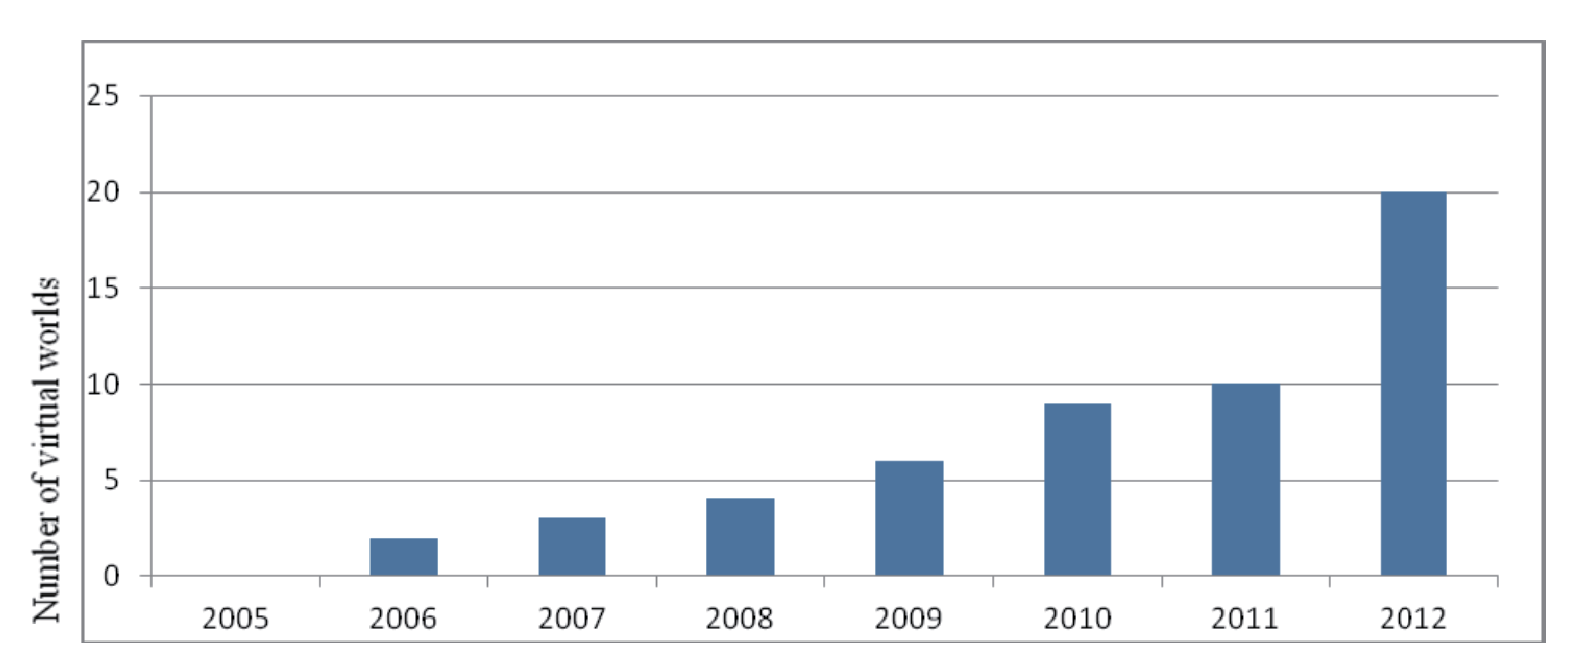
\includegraphics[width=15cm]{eps/vrTrends.eps}
\caption{VirtualRealityのシュミレーション環境の推移}
\label{trends}
\end{center}
\end{figure}

OCULUSは目を完全に覆う没入型の装置で、頭部の動きを3次元トラッキングしてよりインタラクティブでリアルな仮想現実が体験できるようになっている。最近OCULUSはtouchというコントローラーを独自に開発し、仮想空間の中でより直感的な操作を可能にした\cite{touch}。
一方でHTC Viveは70個のセンサーを備え、顔の動きを360度トラッキングできる\cite{vive}。技術はどんどん発展しているがどちらも5万円以上で非常に高額になっている。\\

そこで大衆向けに安価な価格で開発され発売されるようになったのが、Samsung's Gear VR headsetである\cite{samsung}。セッティングも一般ユーザーのために簡単になった。他にもダンボールで作られているGoogleのCardBoardがある。こちらはiPhoneを3Dディスプレーとして使うため2000円で購入が可能である。Cardboard用のアプリの数も増えていて、販売後1ヶ月で1万人が使うようになった\cite{cardboard}。ところがスマートフォンによるVR体験のほとんどはコンサートやローラーコースター、美術館の体験などが多くインタラクティブなものは少ない。\\

またHMDには幾つかの技術的制約があるとOculous VR共同創立者のNate Mitchellが述べている\cite{oculus}。例えば一人称の仮想空間の場合体験者に違和感を感じさせないために身長をユーザーと一致させることで目線を合わせたり、自身の手や足などを拡張空間の中でも作り上げるために全身のトラッキングシステムを考えなかればならない。また物体や空間をよりリアルに見せるために影、テキスタイル、動き、重力や音を正確に表現しなければならならない\cite{vrtrendShiny}。そしてユーザーが乗り物酔いのようにするためには1秒に75フレームのスピードでレンダリングを行わなければならい\cite{HMDifficulties}。UNITYというゲームエンジンなどを使うことでそれらの作業は比較的楽になったがVRコンテンツ制作には声優、デザイナー、アーティストやエンジニアが必要になる。そのためヘッドマウントディスプレーによる仮想空間は多数向けのコンテンツに留まっている。\\

例えば物理的壁を越えて遠くにいる人と会いたい、時間的壁を越えて過去に旅行をした時の思い出を再び体験したい、自ら好きな映画の登場人物となって刺激を感じてみたいと思っても、その人のモデリングデータをまず入力しなければならない。エンジニアリングの知識のないユーザーにとってそういったパーソナルなコンテンツの作成はできないのだ。\\

そこで本研究では新たな種類の仮想現実を体験するための新しい手法として、明晰夢(睡眠中にみる夢のうち自分で夢を見ていることを自覚していながら見ている夢)に着目した。意識することは少ないが人は毎晩睡眠中に人々は仮想現実を体験している。辞書 『大辞泉 第二版』によると、夢とは「睡眠中にあたかも現実の経験であるかのように感じる一連の観念や心像のこと」\cite{dream}と書かれている。\\

明晰夢は1867 年に Saint Denys により研究が行われて以来\cite{saintDenys}、心理学者や哲学者の間で研究が進められてきた。明晰夢の経験者は夢の状況を自分の思い通りに変化させられる、言い換えれば仮想現実を体験することができると語られてきた。 スタンフォード大学博士の Stephen LaBergeは1987 年に The Lucidity Institute を設立し、明晰夢を見るためのステッ プを Mnemonic Induction of Lucid Dreams (The MILD Technique) で紹介した\cite{LaBerge}。しかしThe MILD Techniqueを習得するには特殊な訓練が必要だ。例えば就寝してから5時間たつときにアラームをかけて一度起きて、明晰夢のことを念じながらもう一度寝る。また明晰夢を見るためには、夢を見ているか否かを自覚できる体質にならなければならない。そのためにリアリティーチェックといって、起床中も夢を見ているのか否かを確認する習慣を付けておく必要がある。例えば夢の本数が正確であるかを確認する、口と鼻から息をしっかりしているか確認する、あるいは鏡に覗き込み自分が映るか確認する、ジャンプをして重力を感じるか試すなど、方法は個人によって様々である。他にも夢日記を欠かさず付けて普段から夢を覚えている体質になること。眠りにつく前に体制を正して、深呼吸をし心を落ち着かせる。そして「これから明晰夢を見るんだ」と念じならが寝る。夢で見たい内容を思い浮かべる。MILDは労力が必要で誰もが気軽に始められるものとは言い難い。

\section{研究の目的}
ユーザーの思い出から特定の人物や空間をVRで登場させることはHMDでは難しかった。だからこそ本研究ではHMDに変わって明晰夢に着目する。特別な訓練をしなくても明晰夢を実現できる新しい手法として、レム睡眠・ノ ンレム睡眠かを観測し起きる直前のレム睡眠中にユーザが望む体験に関連のある音を流すスマー トフォンアプリケーションである DreameDate を開発する。\\

明晰夢を促進するデバイスとしては株式会社タカラトミーが開発した夢見工房\cite{takaratomi}やDreamON\cite{dreamOn}などのスマートフォンアプリが提案されているが、どれも商業目的のものが多く信頼性の高い実験データを公開していないため有効性については大いに疑問が残る。そこでDreamDateでは具体的に以下の点を検証したい。

\begin{itemize}
\item 検証1:夢を操作するために効果的な外的刺激の種類
\item 検証2:外的刺激の与え方とタイミング
\item 検証3:ユーザーに精神的・金銭的負担のかからない睡眠観測方法について
\item 検証4:明晰夢を通して仮想現実を体験できるか
\end{itemize}

人生の1/3を過ごす睡眠時間をより有効的に使うことができれば人類の発展に大いに繋がる。これまでにない新しい睡眠のスタイルの実現に貢献したい。

\section{本文書の構成}
第\ref{chap:introduction}章では、本論文を書くに至った背景と目的、そして論文の構成を説明している。第\ref{chap:webapi}章ではユーザーの仮想現実や明晰夢における認識度や要求について事前調査、睡眠中に見る夢の分析を行った。また睡眠観測や明晰夢促進という目線での先行研究や開発事例を述べたのちに、複数の 観点からDreamDateとの比較を行い新しい解決方法について提起する。第\ref{chap:search}章ではDreamDateのプロトタイピングの過程と、システムの概要、利用方法について述べる。第\ref{chap:visualize}章では章では本研究で試作した DreamDateのユーザースタディの結果と考察を述べる。第\ref{chap:coding}章では本研究の総括を行い、また今後の展望について議論する。最後に備考を述べる。
	% 序論
\chapter{研究背景}
\label{chap:webapi}

ユーザーの拡張現実や明晰夢における認識度や要求について事前調査、睡眠中に見る夢の分析を行った。その結果に基づいてDreamtravelerの開発に反映した点について述べる。

\section{拡張現実について調査}
人がどのような拡張現実を望んでいるかを調査するため、理系の学生7人、文系の学生7人、サラリーマン10人、主婦3人を含めた20〜60歳の男女27人にオンラインアンケートをした。これらのインタビュー結果を経て一般的なユーザのニーズを把握し、Dreamtravelerの有効性やDreamtravelerが解決すべき問題について明らかにする。

\subsection{拡張現実を体験するために一般的な人々が支払う金額}
機能性やデザインの詳細を説明した上で、仮想現実を見る手段として次の選択肢から選んでもらった。OCULOUS Rift:85278円、ハコスコ:1500円、iWink:36478円、タカラトミー夢工房:15984円、Dreamtraveler :無料。すると図\ref{userNeedCost}のように、一般的なユーザーの中には拡張現実を体験するためにOCULOUS Riftなどの高額なデバイスを購入しようとする人は少ないということが分かった。ハコスコだと少し数が増えるが、これらのデータから無料で簡単に手に入れることができるツールを多くの人が必要としていることが証明された。

\begin{figure}[htbp]
\begin{center}
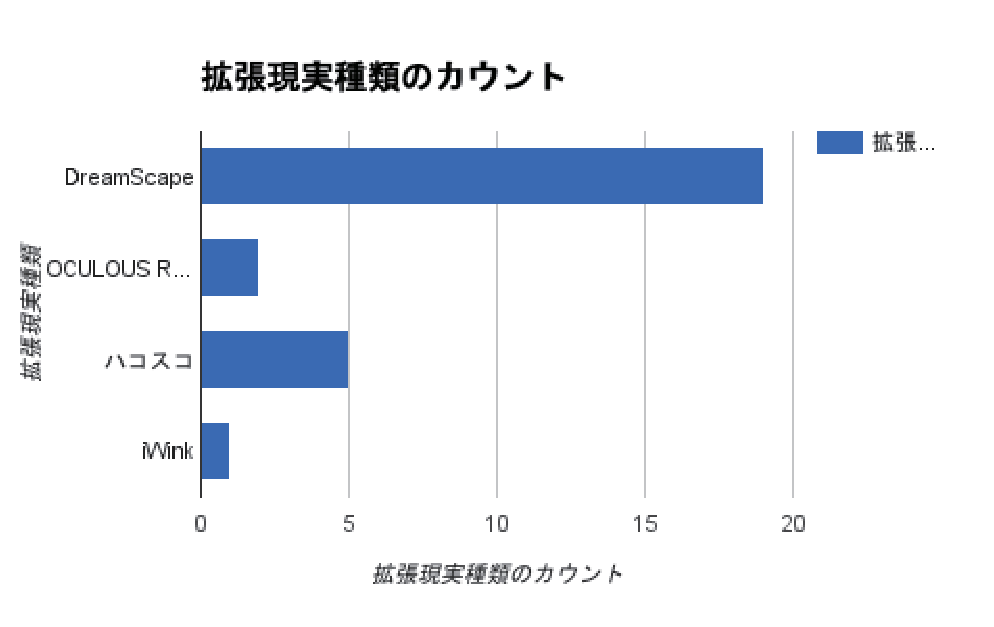
\includegraphics[width=15cm]{eps/VRselection.eps}
\caption{拡張現実を体験するために一般的ユーザーが選ぶ手段}
 \label{userNeedCost}
\end{center}
\end{figure}

\subsection{拡張現実を体験したいタイミング}
拡張現実を体験したいタイミングとして、睡眠中と起きている時間帯でどちらが好ましいかについて調査を行った。すると睡眠中と答えたのは52\%、起床中と答えたのは48\%だった。よって結果にはあまり差がなかった。睡眠中を選択した人は理由として「睡眠時間の有効活用のため」と答えた。比べて起きている時と選択した人は「起きたら忘れてしまうかもしれないから、意識のある時に体験したい」と答えた。よってDreamtravelerの開発において実際に睡眠中の拡張現実がユーザーにどのような体験を与えるかを研究することは意義があると考えられる。


\section{睡眠に関する調査}
\subsection{睡眠段階(睡眠の深さのレベル)と夢}
睡眠は身体を休めるためにある。そして人生の1/3を占める活動である。睡眠中人は2つの睡眠段階、REM睡眠とnonREM睡眠を90分間隔で行き来している\cite{Dement}。REMはRapid Eye Movementの略だ。筑波大と理化学研究所の研究によるとREM睡眠中は記憶形成や脳機能回復の作用がある脳波(デルタ波)が多く見られるというのが通説である\cite{tsukuba}。そしてREM睡眠中は心拍数や眼球の運動が活発化する。REM睡眠の最中に起きたときは夢も比較的覚えている\cite{remNonRem}。一方nonREM睡眠中は脳も身体も休んでいる。\\
 図\ref{SleepHypnogram}は平均的な睡眠のサイクルを示したものである。睡眠に突入して初めてのREM睡眠は10〜12分でもっとも短い。2度目のREM睡眠は15〜20分。最後の夢は15分であるが、通常はアラームなどによって不意に中断されることが多い。平均的に一晩で5〜7回夢をみる。一般的な人生で人は6年間夢を見る。
 夢は環境、時間軸と登場人物がマッチしない場合など、不合理であったり、異様な内容のことが多いが大抵の場合人は夢を見ていることに気がつかない。それは論理的思考力を担う前頭前皮質の機能が低下しているためだ\cite{cortex}。

\begin{figure}[htbp]
\begin{center}
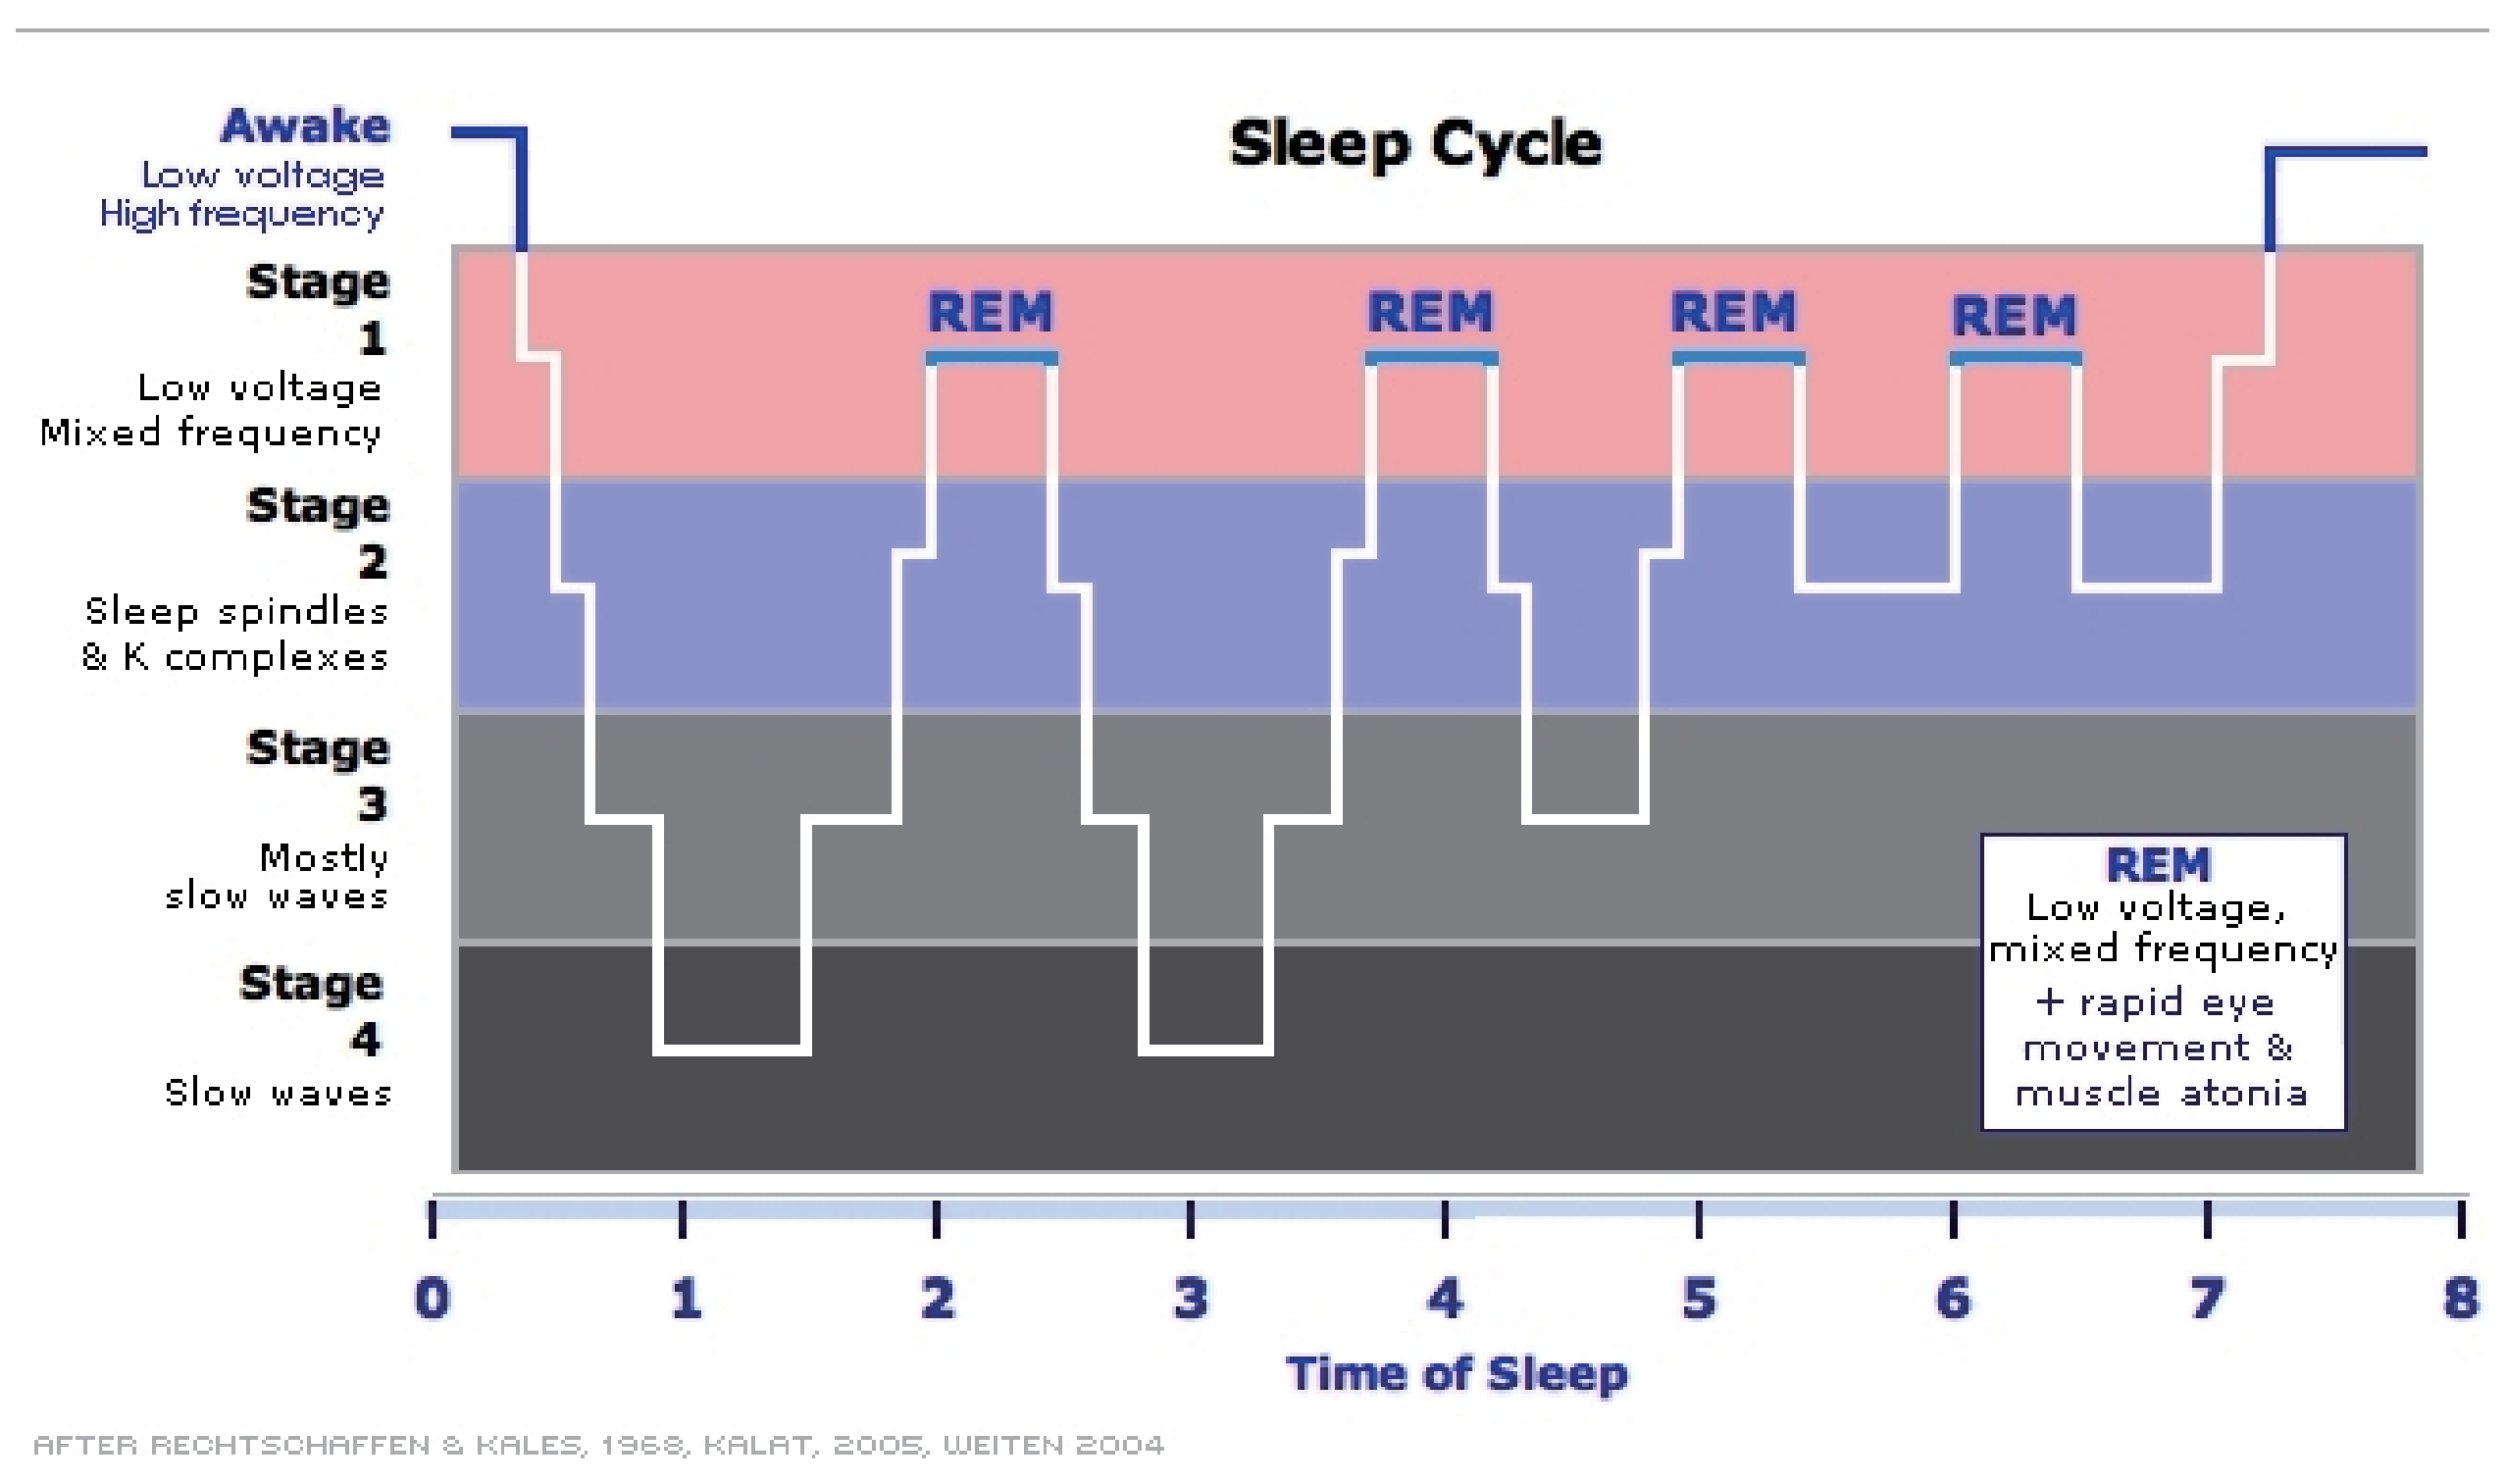
\includegraphics[width=15cm]{eps/SleepHypnogram.eps}
\caption{nonREMとREM睡眠}
\label{SleepHypnogram}
\end{center}
\end{figure}

\subsection{人はなぜ夢を見るのか}
Sigmund Freudによると無意識の欲求や感情、抑圧された子供の頃の記憶、整理的欲求などが影響を与えるという\cite{freud}。Jie Zhangは夢は短期的な記憶を長期的な記憶に変換するためのプロセスであると述べる。具体的には過去の記憶の中で関連性の強い記憶を繋げたり、必要のない記憶を消したりしている\cite{Zhang}。この図\ref{brainZhang}は睡眠中の脳の働きを表す。幼児の平均睡眠時間は16時間でそのう内の50\%をREM睡眠が占める。一方成人の平均睡眠時間は7時間でREM睡眠の長さも短い。年齢が若いほどREM睡眠の周期が長いのは、経験すること全てが新しいため、それだけ多くのことを記憶しなければならないことと、脳の空き容量が多いためと説明されている。

\begin{figure}[htbp]
\begin{center}
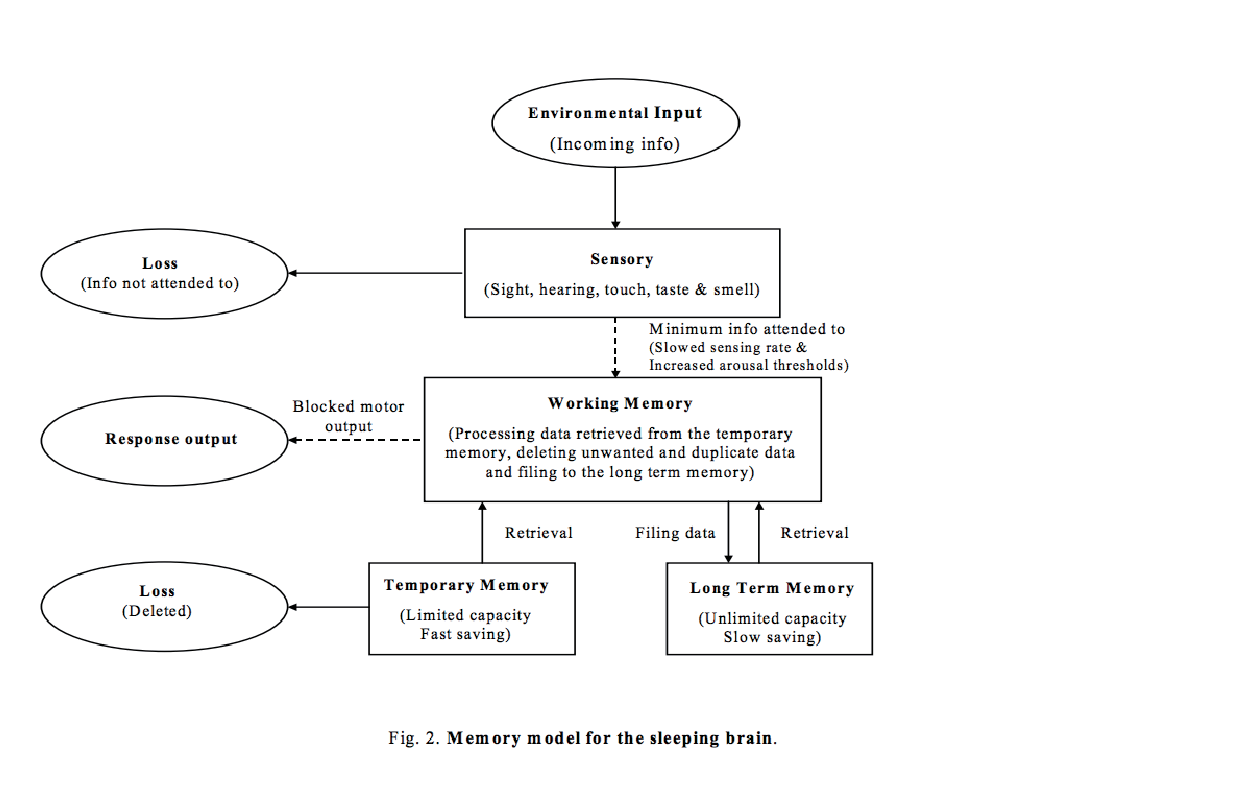
\includegraphics[width=15cm]{eps/sleepBrainModel.eps}
\caption{REM睡眠中の脳の働き睡眠}
\label{brainZhang}
\end{center}
\end{figure}

\subsection{睡眠と寝返りの関係性}
人は睡眠段階を移行させるために寝返りを行う習性があるとされている。要するに睡眠サイクルのスイッチのような働きをする。\cite{negaeri}

\section{明晰夢に関する調査}
\subsection{夢をどのくらい記憶しているか}
夢の操作に成功したとしてもその夢を覚えていなければ意味がない。そこで実験を始める前に一般的に人は夢の内容を起床後どのくらい覚えているのかを調査した。図\ref{rememberDream}がから読み取れるように、夢をよく覚えていると答えた人は少数だった。

\begin{figure}[htbp]
\begin{center}
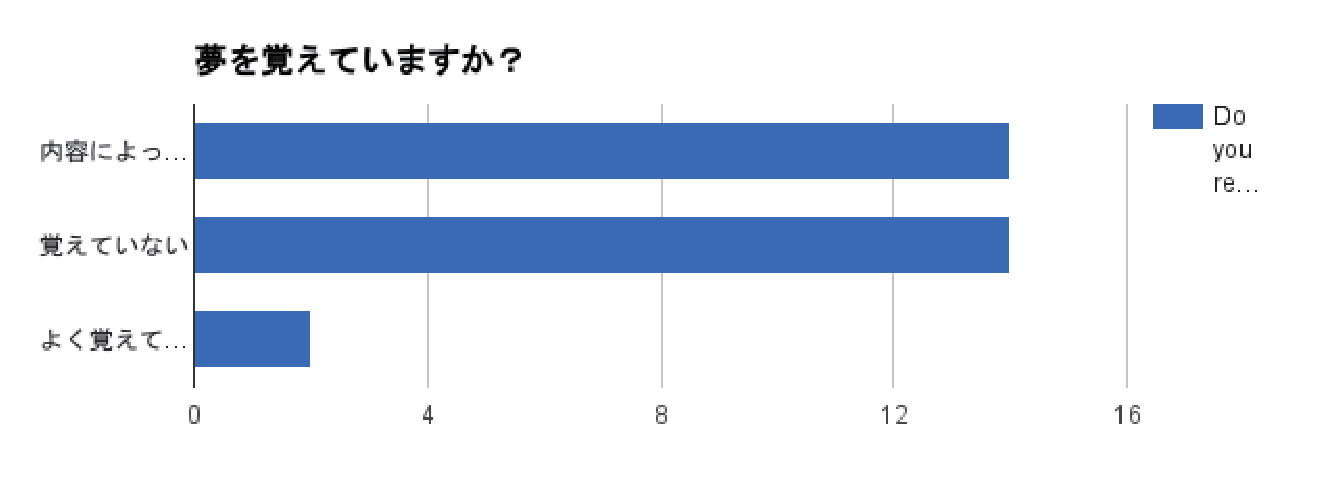
\includegraphics[width=15cm]{eps/remember.eps}
\caption{夢を覚えている比率}
\label{rememberDream}
\end{center}
\end{figure}

覚えている夢は刺激的、怖い夢、繰り返し見た夢というのが多く、日常的な夢は忘れがちであるということが分かった。人は睡眠中の夢の90\%を起床後5分間で忘れるという。Jie ZhangによるとREM睡眠中は短期的な記憶を担っている脳は長期的な記憶への移行に注力していて、インプットの部分があまり機能していないためであると説明する。ただ起きてすぐに、夢日記で夢を記憶すれば覚えていられることが可能なのだ\cite{forgetDreams}。よってDreamtravelerには5分以内に夢の内容を記憶するための日記の機能を加えることに決めた。夢日記は習慣的につけることで効果が出ると言われている。この事実からDreamtravelerの被験者には2週間前から枕の横に紙とペンを置いて起床後すぐに夢の内容を書く習慣を付けてもらうことにした。

\subsection{夢に影響を与えやすい外的刺激}
心理学者フロイトは「夢判断」の中で人は睡眠中の姿勢、環境、身体的刺激によって夢の内容が変化すると述べている\cite{freud}。睡眠中の人間の鼻先を羽毛でくすぐったときに、夢の内容に変化があったことを確認する実験を紹介している。そこで音、体制、匂い、振動、光、などの刺激の中で何が夢に一番影響を与えやすいのかのインタビューで調査をした。以下の図\ref{externalShigeki}がその結果を示す。音が他の刺激よりも影響を与えやすいということが分かった。Dreamtravelerにとって刺激は非常に重要な鍵となるので実験を通してどの刺激が最も有効的なのかを調べた。それについて第3章で述べる。

\begin{figure}[htbp]
\begin{center}
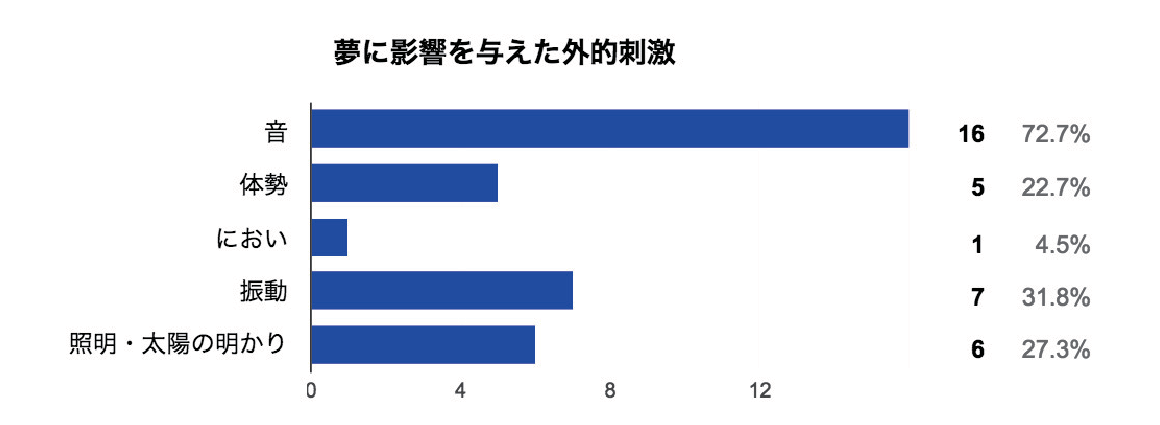
\includegraphics[width=15cm]{eps/input.eps}
\caption{夢に影響を与えた外的刺激}
\label{externalShigeki}
\end{center}
\end{figure}

\subsection{明晰夢のニーズ}
明晰夢を体験したいか否かで質問をしたところ77\%の人が体験したいと答えた。よってDreamtravelerのニーズもあると推測される。

\subsection{明晰夢で体験したい内容}
拡張現実で体験したい内容を調査結果から似ているものをカテゴリー別に分けて、図\ref{desiredDreamTpye}で示した。LOVEタイプ、癒し、元気欲しいタイプ、アドベンチャータイプ、ストーリータイプ、ビジネスタイプとあるがそれぞれの定義を述べる。LOVEタイプとは恋愛や性的行為などが含まれる内容。アドベンチャータイプは冒険など非日常の体験を求める内容。ストリータイプはドラマのように連続性のある夢を求める内容。癒しタイプ・元気欲しいタイプは娯楽を求める内容。原強化タイプは睡眠中になんらかの学習を求める内容だ。LOVEタイプと癒し・元気が欲しいタイプが最も多く、少数派として勉強家タイプがあった。

\begin{figure}[htbp]
\begin{center}
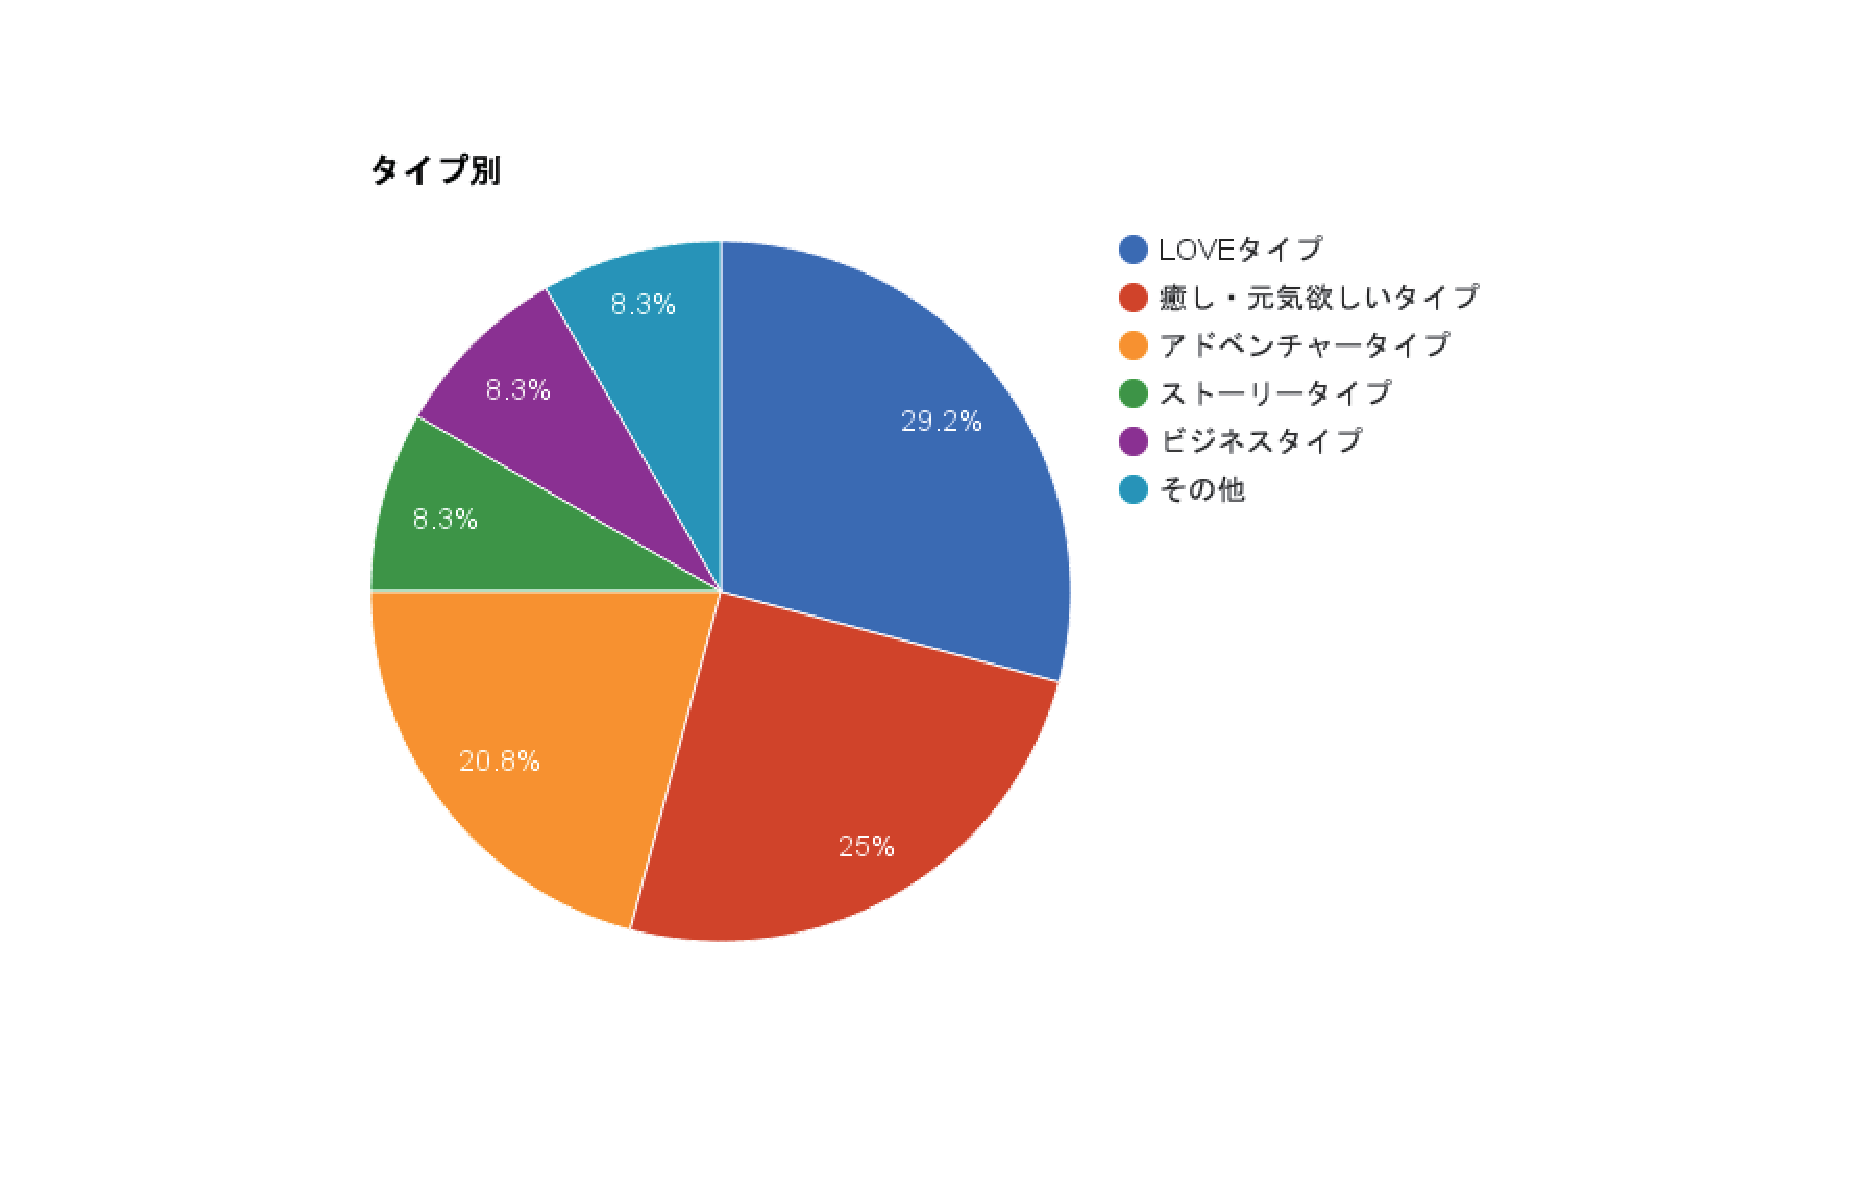
\includegraphics[width=15cm]{eps/dreamType.eps}
\caption{明晰夢で体験したい内容:分析1}
\label{desiredDreamTpye}
\end{center}
\end{figure}

回答をさらに違った方法で分析した結果が\ref{desiredDreamTpye2}である。これらの結果からユーザーによって理想の夢は日常や非日常、具体性や抽象性に隔たりがあり、一貫性が見られないことがわかった。よってDreamtravelerはユーザ一人一人の要望に合った音を選ぶシステムが必要とされることがわかった。

\begin{figure}[htbp]
\begin{center}
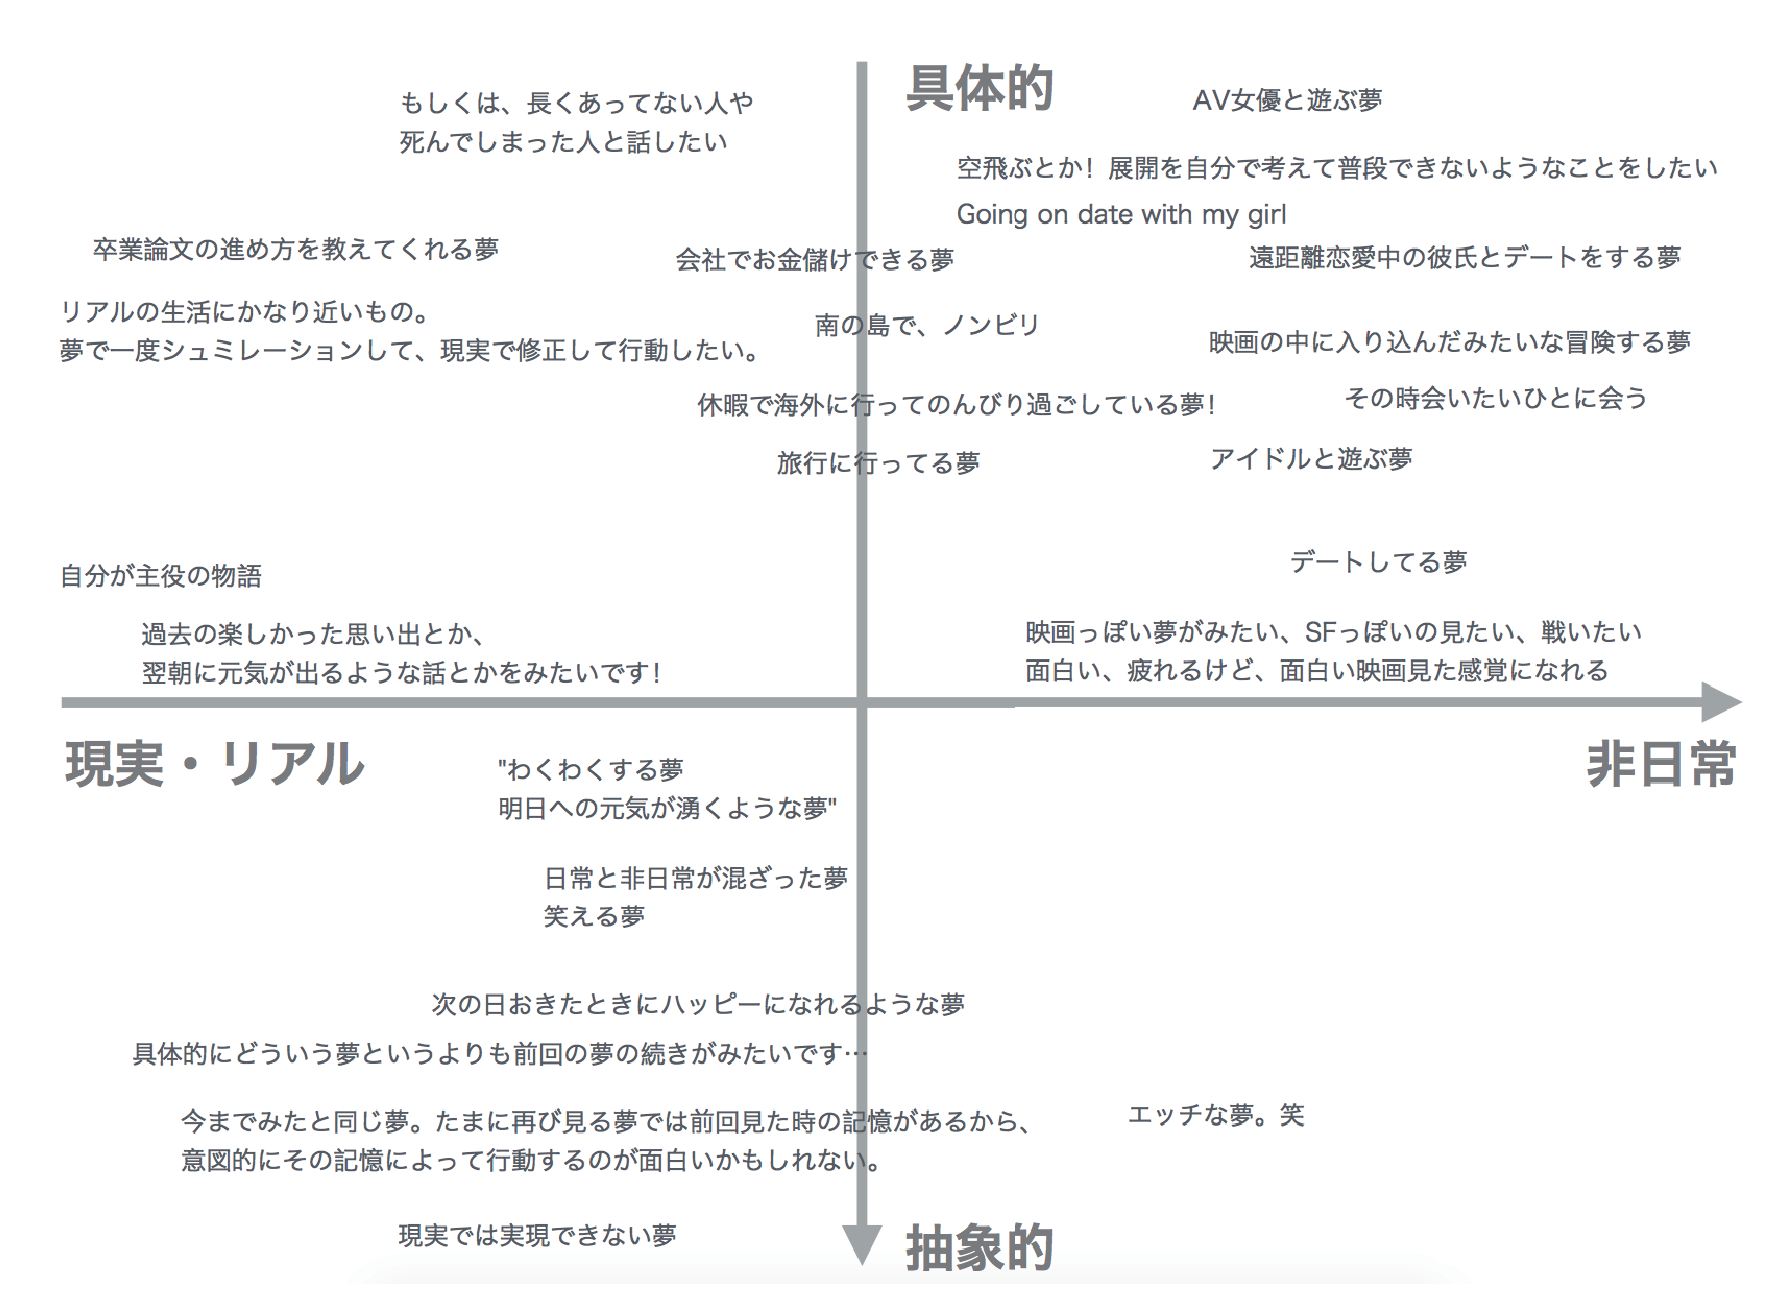
\includegraphics[width=15cm]{eps/whatYouWantToDream.eps}
\caption{明晰夢で体験したい内容:分析2}
\label{desiredDreamTpye2}
\end{center}
\end{figure}

\section{調査から分かったこと}
現実を仮想的に見ることが明晰夢でも可能なのであれば、Dreamtravelerにも興味を示す人が多いということが分かった。明晰夢は睡眠という習慣をより有効に活用し、金銭的コストをかけることなく遂行することができる。求められるのは低価格、高機能、快適なユーザー体験なのでその点に気をつけて開発を進めたい。またコンテンツが見られるようにする対策も必要であろう。	% WebAPIについて
\chapter{DreamDateのプロトタイピングと機能}
\label{chap:search}

この章ではではDreamDateがスマートフォンアプリで睡眠中に音を流すという形に至った背景を述べる。

\section{刺激提示のプロトタイピング}
 人には視覚、聴覚、触覚、味覚、嗅覚を含む5つの感覚器がある。本研究ではそのうちの聴覚と嗅覚による刺激が睡眠中の夢に与える影響を実験を通して観察した。

\subsection{香りによる刺激}
\begin{figure}[htbp]
\begin{center}
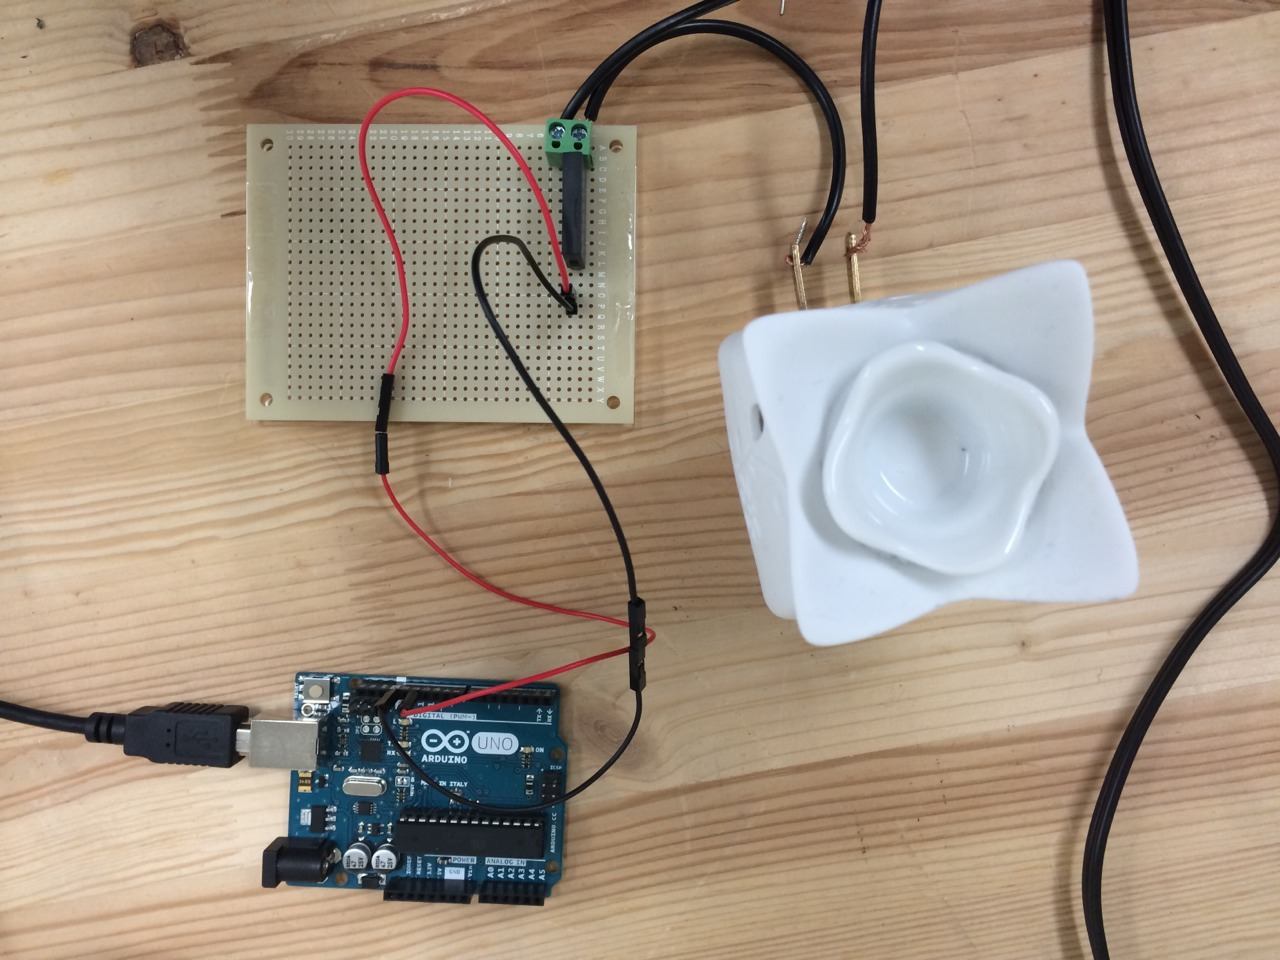
\includegraphics[width=9cm]{eps/smell.eps}
\caption{香りによる刺激}
\label{smell}
\end{center}
\end{figure}

 ラベンダーやバラのような良い香りは睡眠に良い影響を与え、心地良い夢を見やすくするということはMichael SchredlとBoris Stuckの研究によって証明されている\cite{roseDream}。しかし香りが夢の内容に影響を与えるか否かの研究はまだ行われていない。そこでこのプロトタイプはREM睡眠の時に思い出と直結する香りを出して夢を刺激することで夢になんらかの影響を与えられるものか否かを確かめるために製作した。\\
 加速度センサーでREM睡眠を検出したらアロマランプに光がつき、5分後香りが部屋中に充満するという作りになっている。図\ref{smell}にあるのはそのプロトタイプの写真だ。\\
 実験に参加したのは嗅覚が正常に機能している(風邪などを引いていない)22歳の女性3名だ。被験者1には交際相手が部屋で使っているアロマとコーヒー豆の香りで刺激した。被験者2と被験者3はコーヒー豆の香りで刺激した。その香りをたくとすぐに過去の思い出と直感的に繋がる香りをあえて選んだ。またアロマライトは被験者の頭のすぐ横に置いた。\\
 2015年の1月に10日間の実験を行った。香りありの夜、香りなしの夜を5日間ずつ交互に繰り返した。その結果が以下の図\ref{smellExperiment}の通りだ。

\subsection{音による刺激}
 同じ被験者に今度は香りではなく音によるインプットをしてもらった。REM睡眠中に海の音や交際相手と一緒に聞いた音楽を流した。すると音によっては起こされてしまったり、被験者によっては全く影響が出ないという結果になった。しかし、図\ref{smellExperiment}が示すように、香りのインプットでは影響が全くなかったのに比べ、音のインプットは被験者1、被験者2ともに音による刺激で1日だけ夢を観たことがわかった。

\begin{figure}[htbp]
\begin{center}
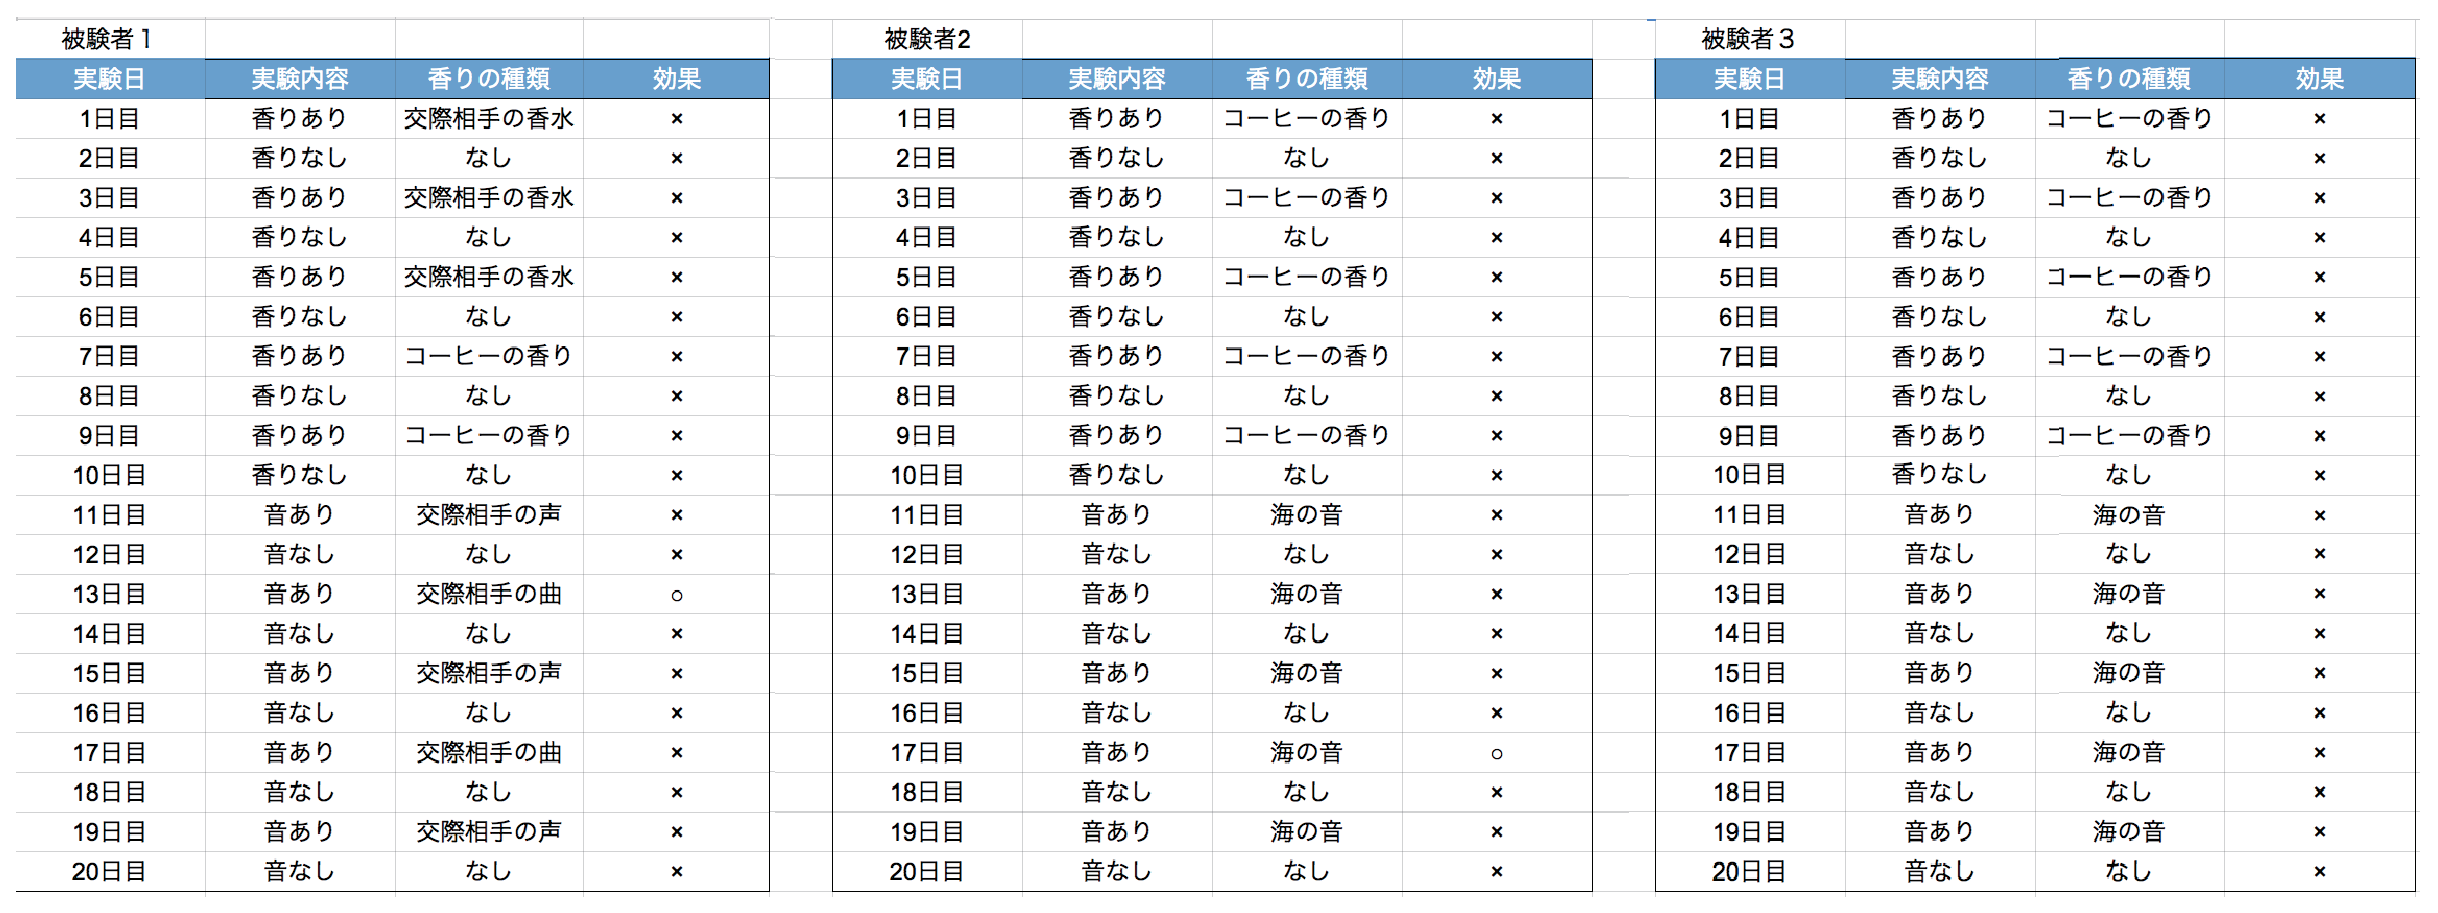
\includegraphics[width=15cm]{eps/smellExperiment.eps}
\caption{香りによる刺激の実験結果}
\label{smellExperiment}
\end{center}
\end{figure}

\section{睡眠観測のプロトタイピング}
ユーザーの睡眠深度のモニタリング方法はいくつかある。それぞれの方法をユーザビリティと機能性の2つの観点から、実験を通して分析する。

\subsection{脳波センサーによる観測}
 このプロトタイプではNeuroSkyのThinkGear ASICモジュールという脳波センサーを使用した。Theta波が4〜7.2HzかつDelta波が0.5〜4Hzである時をREM睡眠中であるとし自らが実験台となり装着して寝てみた。しかしこの手法は頭を締め付けられる感覚があり、且つ汗をかいてしまうのでユーザーに負担がかかる。寝心地を損ねてしまうということがわかりセンサーの体と離す別の方法を試すことにした。
\begin{figure}[htbp]
\begin{center}
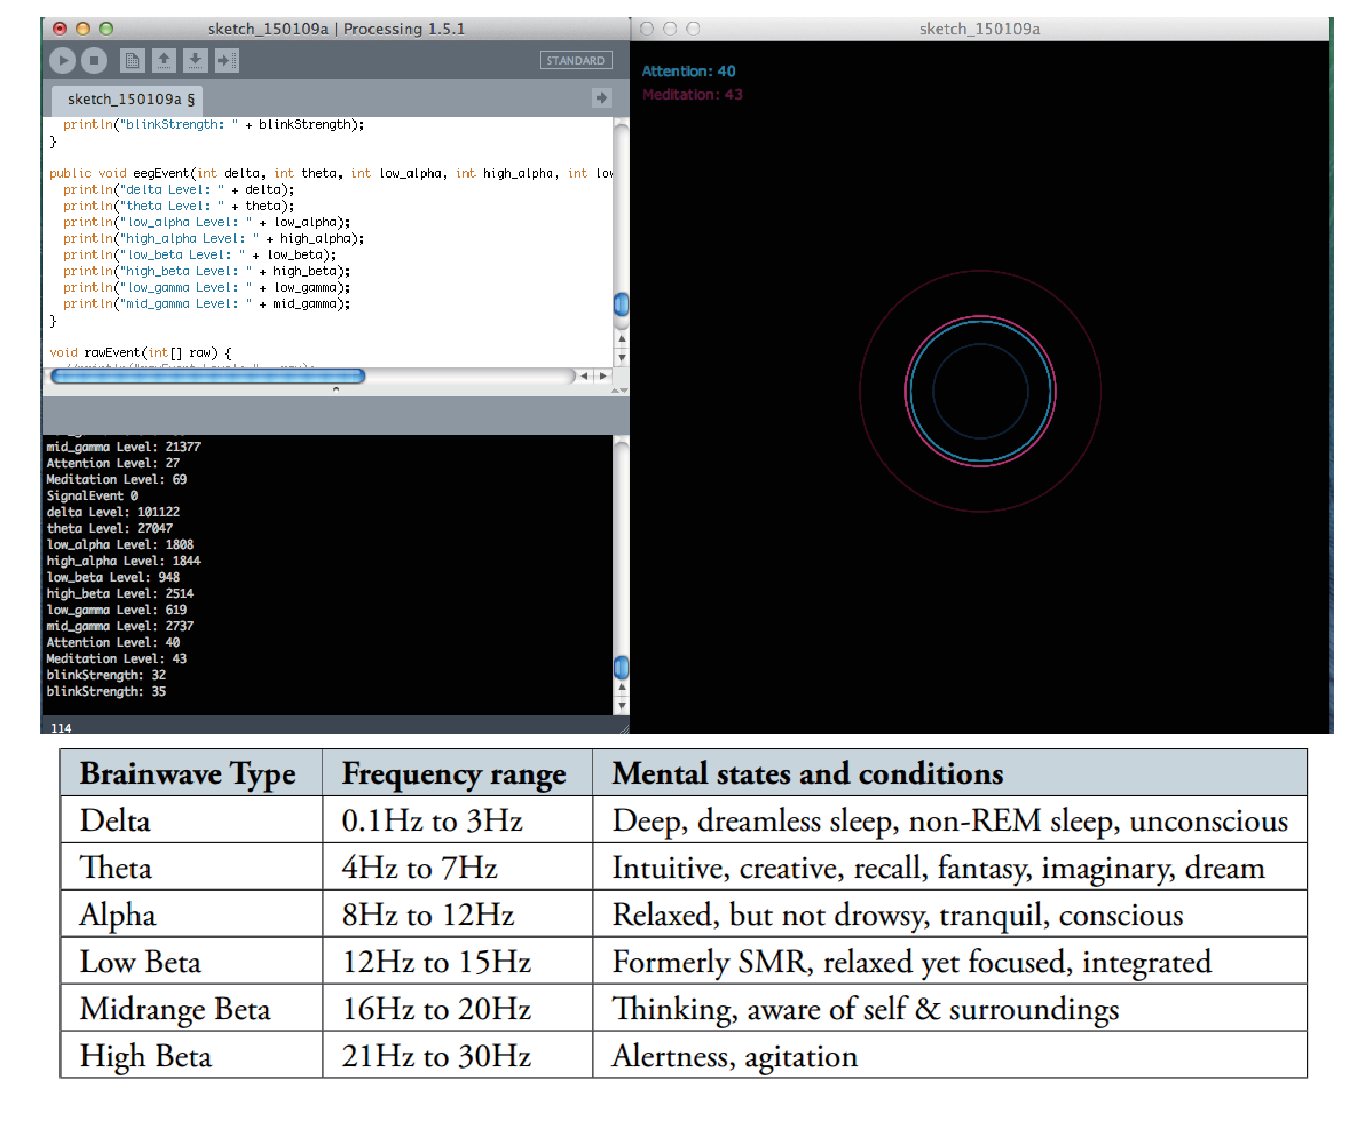
\includegraphics[width=10cm]{eps/brainWave.eps}
\caption{脳波センサーによるセンシングのプログラムと睡眠ステージと脳波の数値}
\label{brainWave}
\end{center}
\end{figure}

\subsection{心拍センサーによる観測}
 次に市販で売られている心拍センサーを追懐睡眠中の心拍数を観測することでREM睡眠を検出できるかどうかの実験をした。しかし寝ているときに指にセンサーを装着するのは発汗のを引き起こし、ユーザー体験の視点から非常に好ましくないということがわかりまたしても別の方法を試すことにした。

\begin{figure}[htbp]
\begin{center}
\includegraphics[width=10cm]{eps/heart.eps}
\caption{心拍センサーによるセンシング}
\label{heart}
\end{center}
\end{figure}

\subsection{kinectによる観測}
 このプロトタイプはKinectを使用して、ユーザーの寝返りを検知して音楽を流すシステムである。図\ref{kinect}のようにkinectを天井に設置する。ウェラブルセンサーではないためユーザには負担がかからない。但し布団をかぶってしまうとkinectによる骨格トラッキングは難しい。そのためOpenCVのライブラリを利用して、画像処理を行った。\\
 寝返り判定の正確性を確かめるために、実際にベッドの上で寝返りを打ったとき音が鳴るかを試したところ、開発したプログラミングではノイズが多く出て誤作動が起きてしまうのでkinectを使うのは適切ではないと判断した。しかしプログラミングの能力が高い人により開発されれば、kinectによるトラッキングの精度もあげられるはずである。ただし、デバイス自体の価格が高いのと、取り付けに労力が必要とされることと、ポータブルではないため旅先では使えないという点で、本研究では好ましくないとした。

\begin{figure}[htbp]
\begin{center}
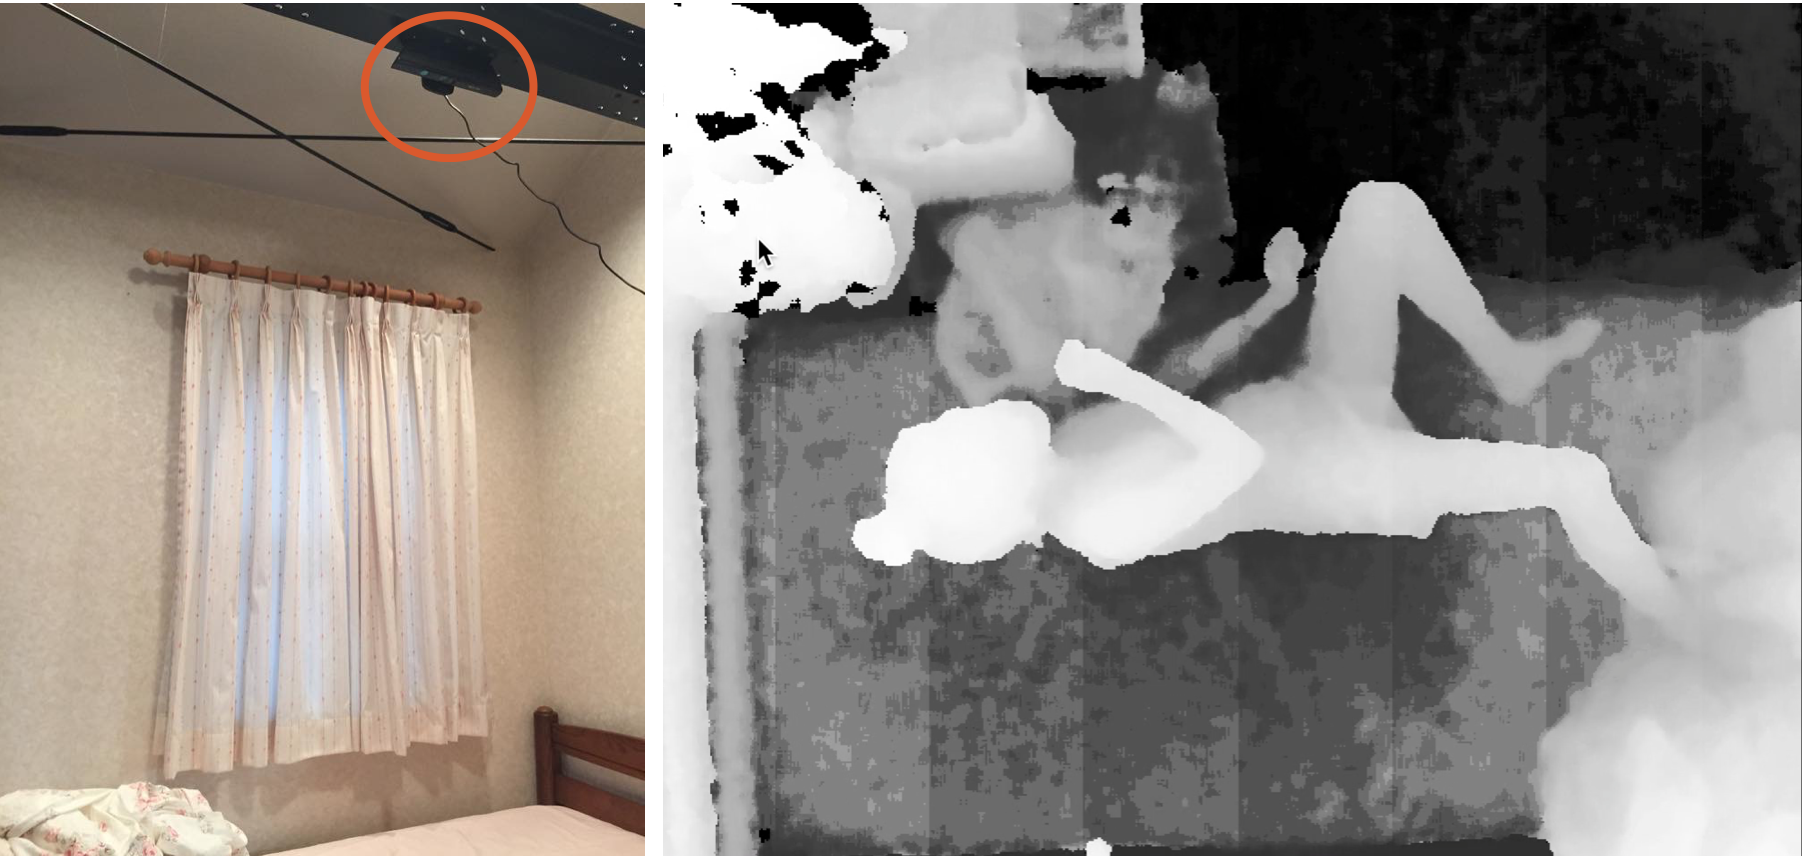
\includegraphics[width=15cm]{eps/kinect.eps}
\caption{kinectによるセンシング}
\label{kinect}
\end{center}
\end{figure}

\subsection{スマートフォンの加速度センサによる観測}
 最終的に多くの人々が既に使用していて、ユーザビリティーの視点から見てもっとも負担のかからないスマートフォンアプリケーションによるセンシングに試みた。スマートフォンで計測すときはウェラブルではないため身軽であるし、持ち運びが簡単なので旅中も使える。スマートフォンアプリケーションによるセンシング方法とその正確性については5章で述べる。

\section{実装}
\subsection{機能}
 現在、仮想現実を体験すべくヘットマウントディスプレーなどの様々なツールが開発されている。そこで睡眠中の夢を自由自在にコントロールする方法があれば誰もがより簡単に仮想現実を体験できるのではないかと考えた。\\
 睡眠中にユーザーがの思い出と関連した音を流すことで、その音に基づいて夢を見ることを促進するスマートフォンアプリDreamDateを試作した。ターゲットと考えているユーザーは日々のストレスから解放されたい人、懐かしい思い出をもう一度体験したい人、物理的に会えない人と会いたい人などだ。\\
 DreamDateには3つ主要な機能がある。一つ目は寝る前に印象に残っている記憶に関する写真と映像を表示する機能。二つ目は睡眠中にREM睡眠を検出し、記憶を連想させる音を流す機能。例えば特別な誰かを連想する音、旅行中によく聞いていた曲、最寄り駅の音楽、好きな映画のサウンドトラックなどだ。三つ目は起床後に夢について記録する夢日記機能である。ユーザーには睡眠前にスマートフォンを画像\ref{DreamDateImage}のように枕の横に置いてもらう。\\
 アプリを使用して実験をした結果、DreamDateには欠点があることがわかった。それはユーザーが自分の記憶を連想する音を探し出して登録しなければならないということ。例えば海の音を聞けば海の夢を見れるということではないのだ。しかし実際に海に行った特別な記憶がある人であれば、海の音を流せばその夢を見る確率は比較的に上がる。\\
  DreamDateは開発途中でまだAppストアには掲示していないが、githubからソースコードを入手することができる。iOSスマートフォンを持っていて、Apple Developerの登録をしている人であればインストールできるようになっている。

\begin{figure}[htbp]
\begin{center}
\includegraphics[width=14cm]{eps/dreamDate02.eps}
\caption{DreamDateの配置}
\label{DreamDateImage}
\end{center}
\end{figure}


 Xcode 上で openframeworks ライブラリを利用して、iPhoneの加速度センサーを利用した体動検知アプリケーションを制作した。睡眠時に枕の横に iPhone を置いて、体動(寝返り)による寝具の動きを検知して加速度を測定す る。\\

 まずベッドの硬さは人により違うため、キャリブレーションをしてもらう。アプリ起動後ユーザーにはiPhoneを横に置いた状態で15秒間静止してもらう。x軸の加速度を毎秒記録、1秒前の加速度との差分を導き出す。20秒間、x軸の差分の中での最大値を閾値として設定する。y軸とz軸の測定をしなかったのはx軸だけでも十分寝返りを特定できるためである。\\

 ベッドで寝てから睡眠に至るまで平均的に10分から20分かかるとされているため、スタートボタンが押されてから20分後に加速度センサーによる体動のモニタリングが開始される。こうすることで、寝ようとしている最中に音楽がならないようにする。モニタリングが開始されてからはノイズを除去するために、毎20秒の平均値が出される。その平均値が閾値に比べて高くなった時に寝返りをしたと判定する。寝返りを打つ時は睡眠段階がREM睡眠からnonREM睡眠に、あるいはnonREM睡眠からREM睡眠への切り替わったときだ\cite{negaeri}。そのためREM睡眠の間はあらかじめ設定していた音楽が図\ref{melodyGraph}で示したオレンジのタイミングで流れる。REM睡眠時にのみ音楽を流したのは常に音楽が流れていると睡眠が害され睡眠サイクルが崩れて体調不良などを引き起こす可能性が高くなるためだ。

\begin{figure}[htbp]
\begin{center}
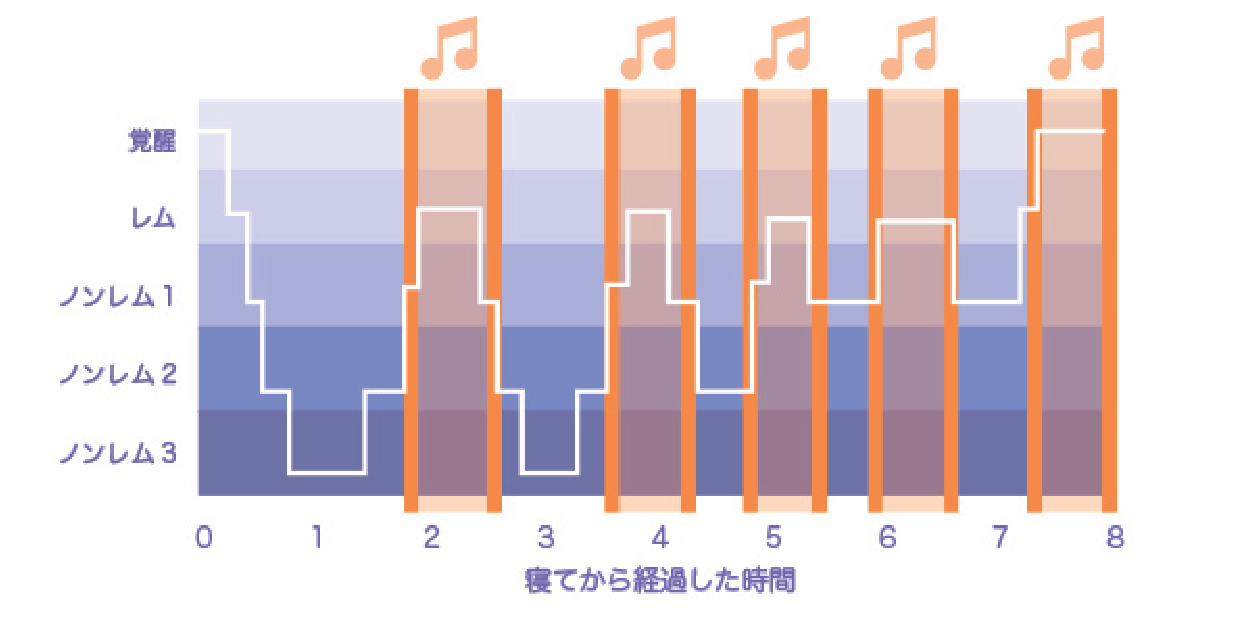
\includegraphics[width=15cm]{eps/remNonrem.eps}
\caption{音刺激提示のタイミング}
\label{melodyGraph}
\end{center}
\end{figure}


一晩中のx軸の数値、音楽の再生状況、夢日記の結果はデータベースをクラウドであるParseに保存する。図\ref{system}に一連のプログラムの流れを記載する。
\begin{figure}[htbp]
\begin{center}
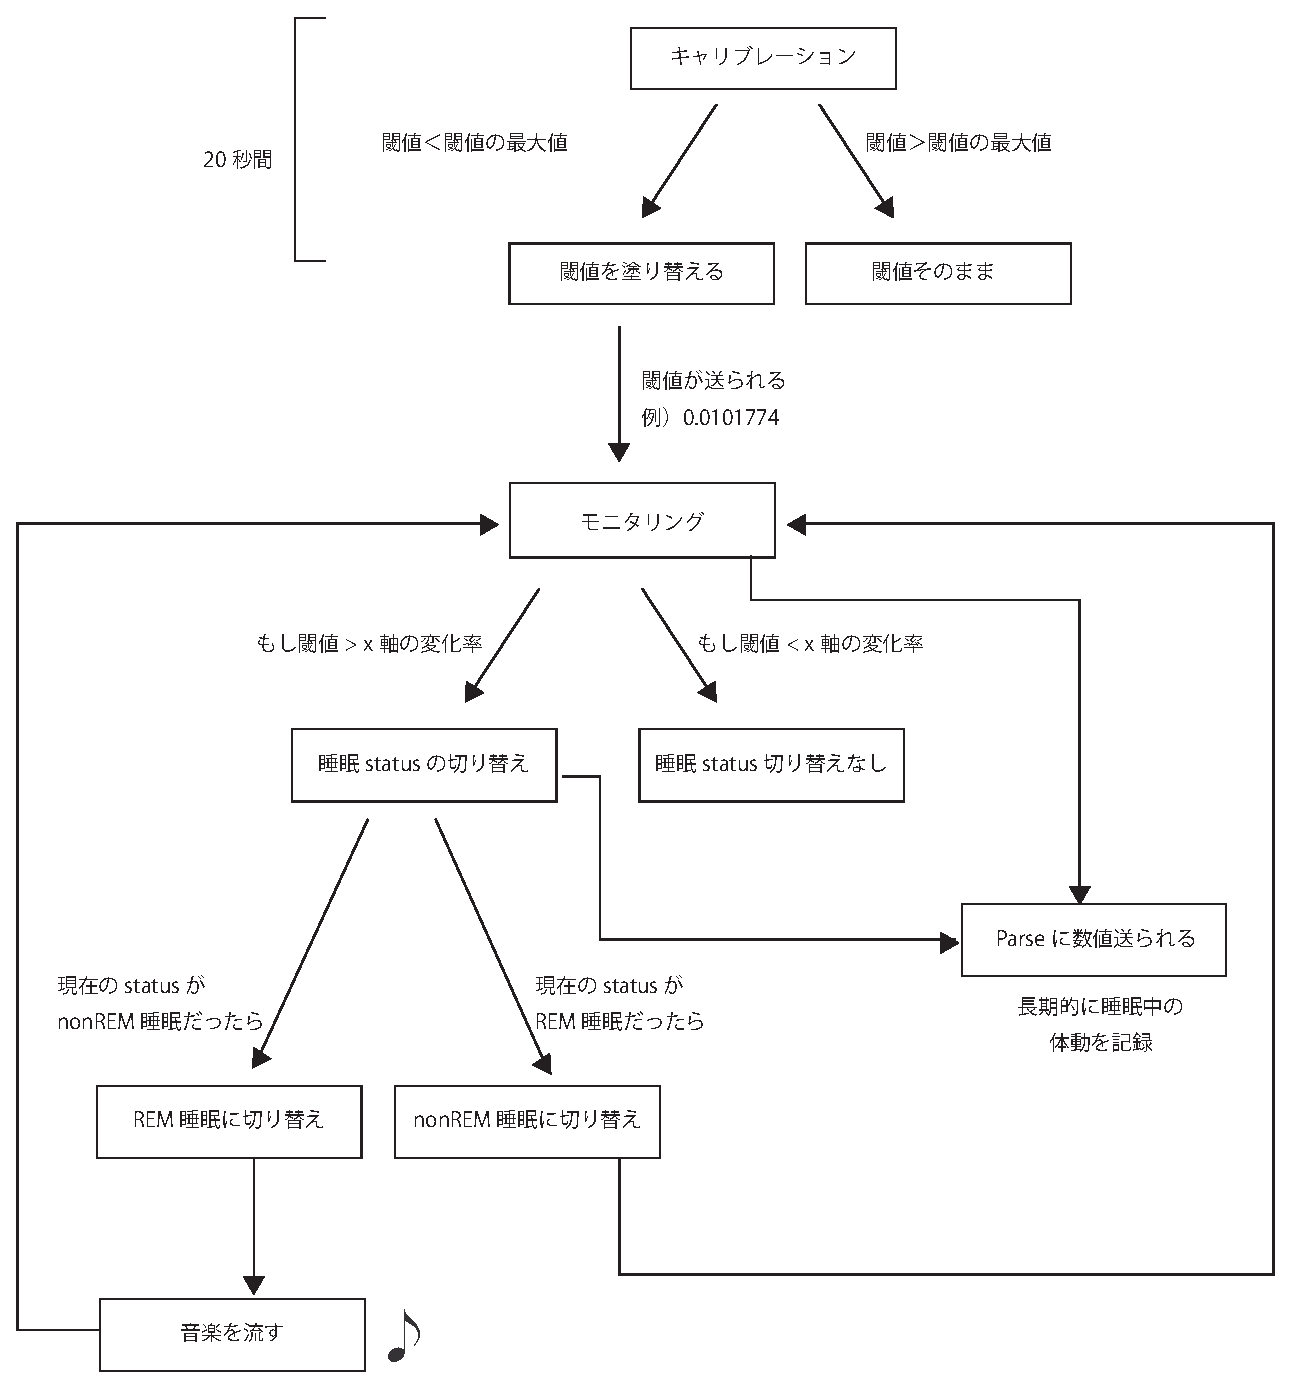
\includegraphics[width=15cm]{eps/system.eps}
\caption{DreamDateのフローチャート}
\label{system}
\end{center}
\end{figure}

\subsection{利用方法}
 ユーザーには予め記憶を思い起こさせる音と画像を登録してもらう。音選びは適している音声と適さない音声があるため注意する必要がある。使用してはいけない音は人の声だ。特に喋りかけてくるような内容の音声は、ユーザーを起こしてしまう可能性が高いということが実験結果から分かった。詳しくは第6章で述べる。逆に適している音は繰り返しある環境下で聞いていた音である。
 アプリの起動後、\ref{le01}のような画面が表示される。そこには「自動ロック機能をOFFにする」「音量は1〜3に設定する」やiPhoneの置く位置などの指示が書かれている。次に\ref{le02}の画面に遷移し、ユーザーの思い出に関連性のある画像を表示する。ここでは寝る前に記憶の情景を思い出す機会を与えている。そして\ref{le03}の画面では思い出の音楽が流れる。音楽を聴きながら、旅先での空間、香り、音の細部までを思い出して、気持ちを落ちつかせて瞑想状態に入ってもらう。次に\ref{le04}の画面に移動する。ユーザーは寝る前にアプリを起動してスタートボタンを押し、起動させたままスクリーンを伏せて枕の横に置く。20〜30分間後にDreamDateの加速度が起動をし一晩中ユーザーの体動のトレッキングが行われ、REM睡眠を検知すると音楽がなる。起床後\ref{le05}の画面で、ユーザーは起床すると夢の内容を忘れないように日記に投稿する。

\begin{figure}[htbp]
 \begin{minipage}{0.45\hsize}
  \begin{center}
   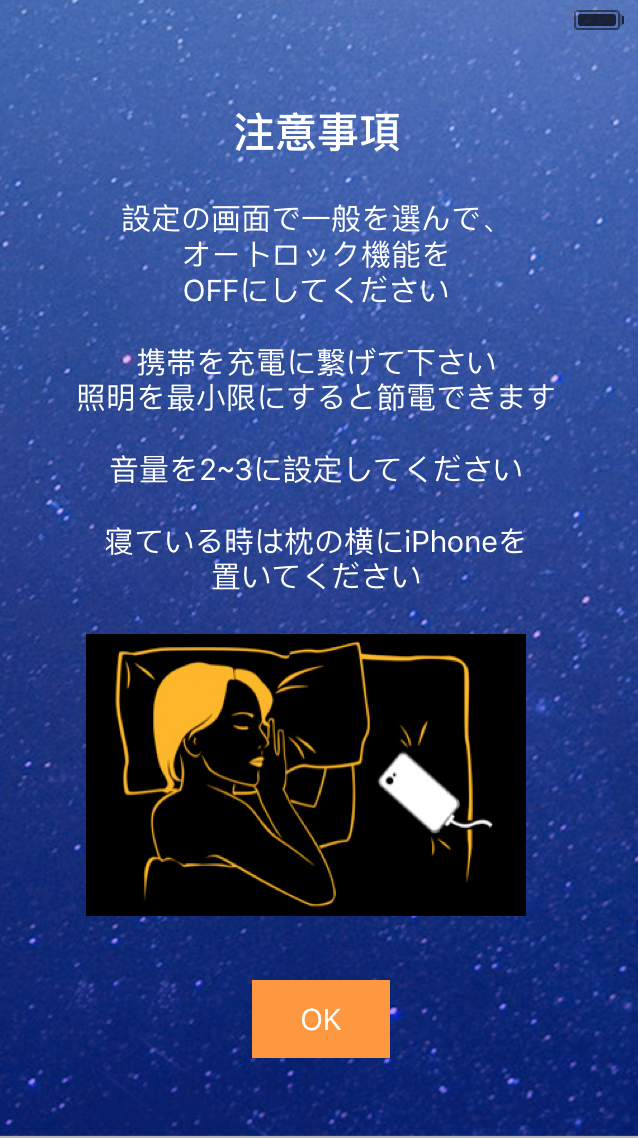
\includegraphics[height=90mm]{eps/AppIntro.eps}
  \end{center}
  \caption{起動画面}
  \label{le01}
 \end{minipage}
 \begin{minipage}{0.45\hsize}
  \begin{center}
   \includegraphics[height=90mm]{eps/AppMemoryImages.eps}
  \end{center}
  \caption{思い出の画像を表示}
  \label{le02}
 \end{minipage}
\end{figure}

\begin{figure}[htbp]
 \begin{minipage}{0.45\hsize}
  \begin{center}
   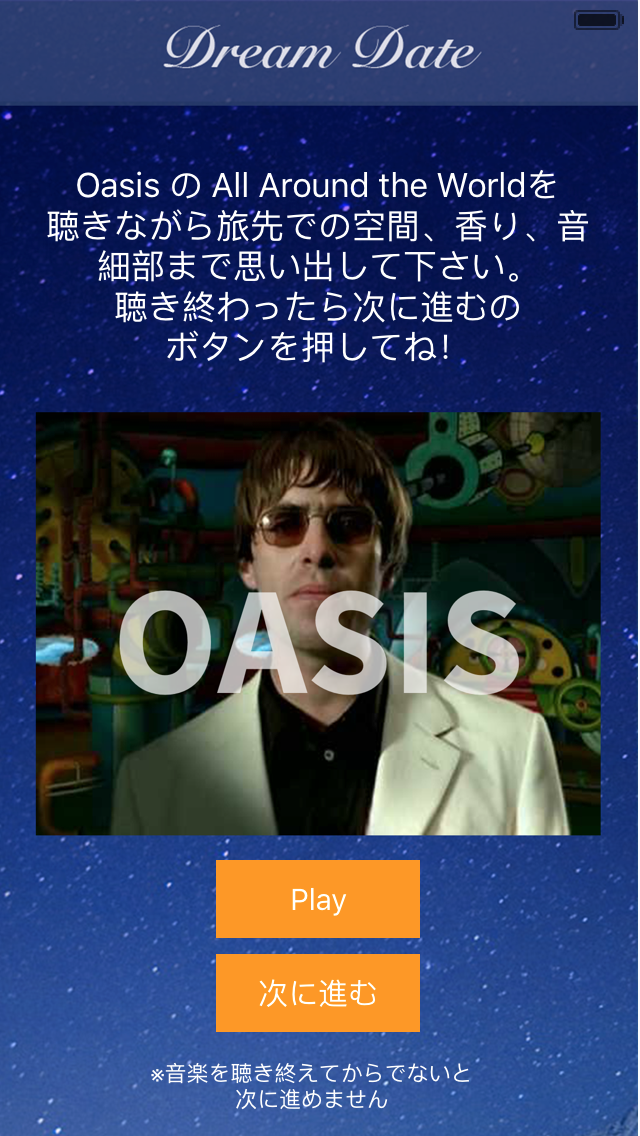
\includegraphics[height=90mm]{eps/AppMusicPlay.eps}
  \end{center}
  \caption{思い出に関連した音刺激の提示}
  \label{le03}
 \end{minipage}
 \begin{minipage}{0.45\hsize}
  \begin{center}
   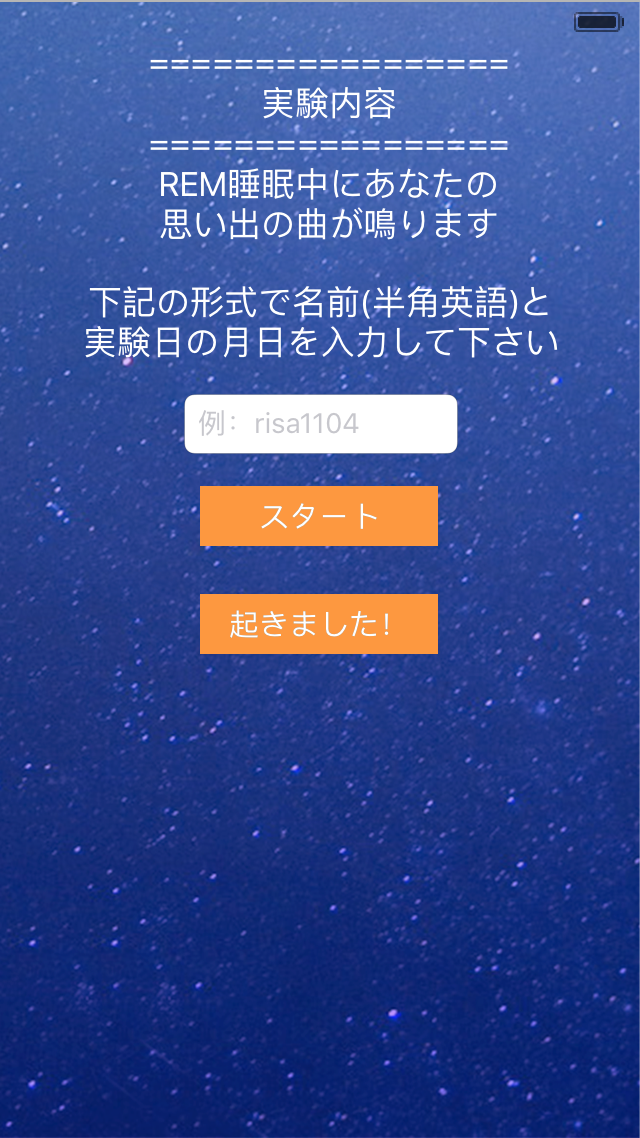
\includegraphics[height=90mm]{eps/AppStart.eps}
  \end{center}
  \caption{睡眠開始ボタン}
  \label{le04}
 \end{minipage}
\end{figure}

\begin{figure}[htbp]
 \begin{minipage}{0.45\hsize}
  \begin{center}
   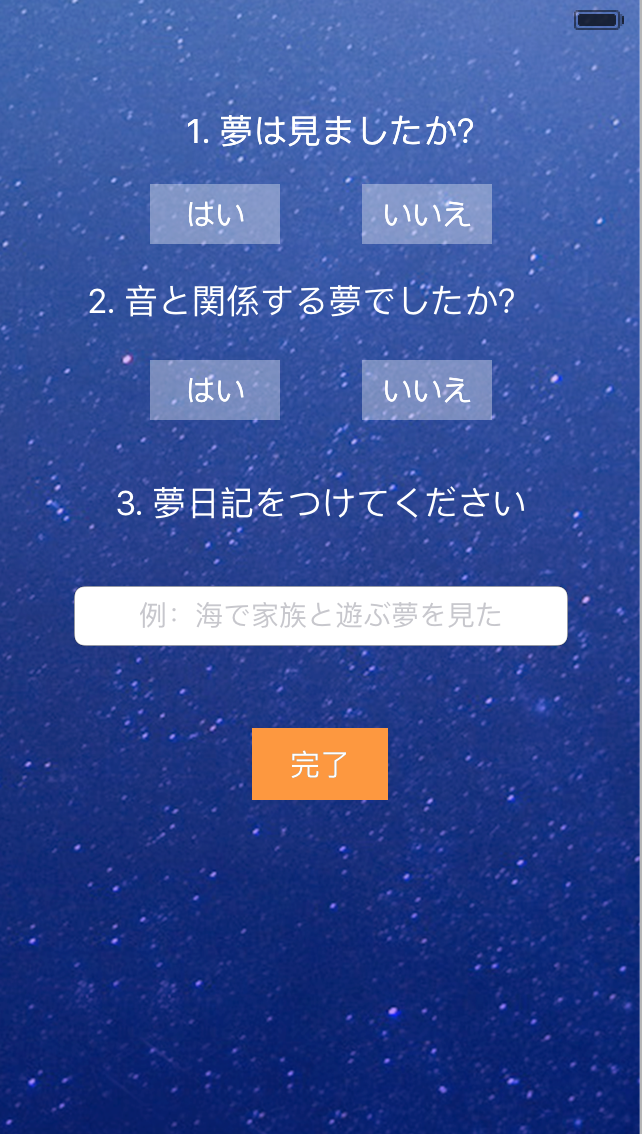
\includegraphics[height=90mm]{eps/AppDiary.eps}
  \end{center}
  \caption{夢日記記入ページ}
  \label{le05}
 \end{minipage}
 \begin{minipage}{0.45\hsize}
 \end{minipage}
\end{figure}
	% 検索エンジンの精度向上
\chapter{ユーザスタディ}
\label{chap:visualize}

本章では開発したスマートフォンアプリDreamDateを用いたユーザスタディとその結果について述べ、提案手法の長所及び短所について考察する。

\section{予備実験1:音刺激の有無}
寝る前の10分間とレム睡眠中に曲を流すことが夢に影響を与えるか否かを検証するため予備実験を行った。スマートフォンは充電をした状態で枕の横に置くことで音が脳に届く状態にした。また睡眠を始める前に5分間海の夢が見たいと被験者に念じてもらった。\\
 20代後半女性の被験者A、40代後半女性の被験者Bと、20代前半女性の被験者Cに海の音を聞く日と効かない日を交互に14日間続けてもらうことで音が夢に影響を与えるのか否かの記録を行った。14日間の実験を行ったのは睡眠に関する実験は体調その日の活動内容や被験者の心境によって左右され、データーが変動しやすいためである。図\ref{experiment1}が実験スケジュールと実験結果である。青のハイライトがある日が関連する夢を見た日である。音が無い場合に被験者が海の夢を見たのは1回なのに対し、海の音を流して海の夢を見たのは4回であった。\\
 夢の具体的な内容について実験後インタビューをした。すると3日間夢を見たと答えた被験者Aは音のインプットが無い日は会社で働いている夢を見ることが多く、音を流しながら寝た日は10日ほど前に行った沖縄旅行での夢を見たと答えた。一度も海に関連した夢を見なかった被験者Bは海の音で起こされたりしたため、音は流れていたが全く関係の無い夢を見たと答えた。被験者Cは実験の最後の方で1年前に旅行したアメリカ西海岸に関する夢を見たと答えた。

\begin{figure}[htbp]
\begin{center}
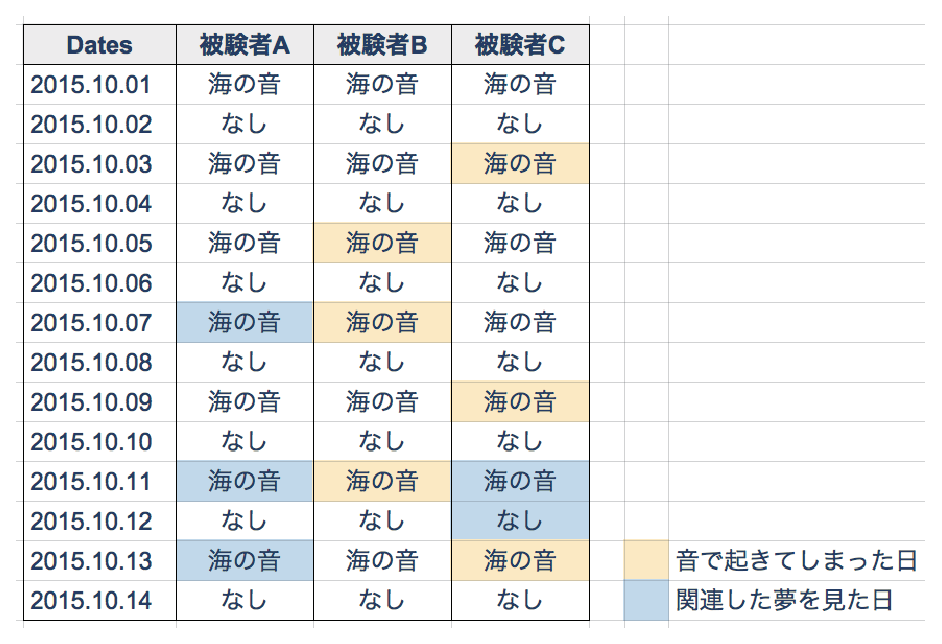
\includegraphics[width=13cm]{eps/schedule0.eps}
\caption{予備実験1:実験スケジュールと実験結果}
\label{experiment1}
\end{center}
\end{figure}

\section{予備実験2:音刺激の種類}
 どのような音がDreamDateに適しているのかを調べるために予備実験を行った。2年前から遠距離恋愛中の交際相手とデートをしている夢を見たいと望む被験者Cに「音声」、「曲」と「自然音」の3種類の音を試した。被験者Cの場合は「音声」は交際相手が被験者Cの名前を語りかけ、過去のデートの思い出話や、理想のデートの話しや、愛の言葉をささやくといった内容であった。「曲」は交際相手が被験者Cのために作曲と演奏した曲で、被験者Cも毎日通学で聞いている曲である。「自然音」はアメリカ西海岸の海で交際相手と共に聞いた波の音。図\ref{experiment2}が実験スケジュールと実験結果である。被験者の希望であった遠距離恋愛中の交際相手とデートしたいという要望を実現させることができたのは「曲」であった。\\
 夢の具体的な内容について実験後インタビューをした。関連する夢を見たのは「曲」と「自然音」のときである。11月9日は日本で再開する夢をみて、11月13日は江ノ島で友人と遊ぶ夢をみた。11月15日は交際相手から手紙が届く夢を見た。また、実験の結果から語りかけ口調の音声は被験者を毎回起こしてしまった。比べて波の音などの自然音や音楽は比較的被験者を1度しか起こさなかった。

\begin{figure}[htbp]
\begin{center}
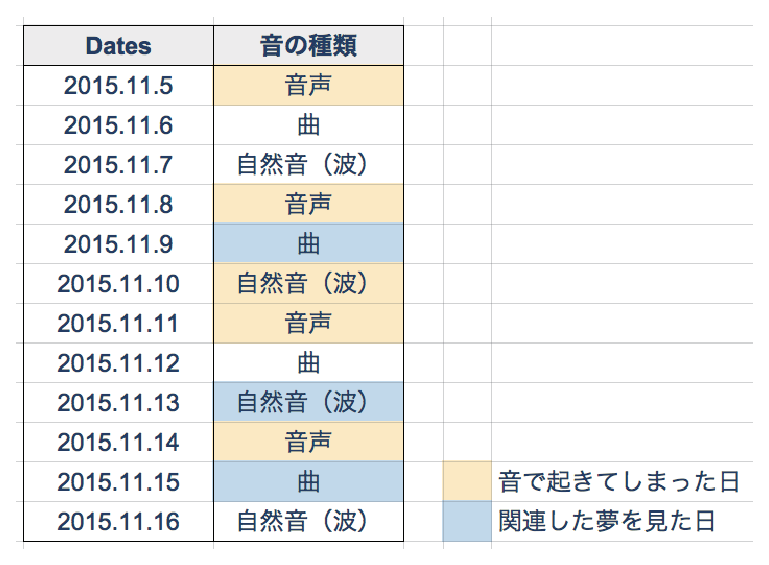
\includegraphics[width=13cm]{eps/schedule1.eps}
\caption{予備実験2:実験スケジュールと実験結果}
\label{experiment2}
\end{center}
\end{figure}

\section{予備実験から浮かび上がった仮説}
 予備実験1を経て同じ海の波の音でも結果に個人差が出るということがわかった。その理由として考えられるのがまず年齢である。Zhangは高齢になるにつれてレム睡眠の間隔が短くなると述べている\cite{Zhang}。次に考えられるのが被験者がどれだけそれに関連した夢を見たいと感じているかである。海の音を流した夜、被験者には全員海の夢を見たいと念じながら寝るようにと伝えたが、本心として海の夢を見たいと思っていたのは被験者Aと被験者Cのみであった。夢に対する希望が大きいほど、夢を見る確率が上がる可能性がある。他にも要素として考えられるのが、音と被験者の記憶との関連度だ。実験を行った後にそれぞれの被験者にどのような夢を見たかインタビューをした。すると海の夢を見た被験者 A と被験者 C はどちらも過去に海に行った際の思い出を夢見たと答えた。一方で 海にしばらく行っていない被験者 B は一度も海の夢を見なかった。この結果は被験者の記憶と関連性の高い音を流すと効果が出やすいということが示唆する。言い換えると印象に残っていない 体験や情景を DreamDate を使っても夢で再現することは困難である可能性がある。最後にどDreamDateの使用日数が結果に影響を与える可能性がある。というのは被験者Aと被験者Cは共に実験の前半に比べて実験後半の方が夢をみる確率が上がっているからである。明晰夢習得へのステップであるThe MILD Techniqueでも訓練を長く続ければ続けるほど、成功率があがると紹介されていることからDreamDateもな学使えば使うほど効果が出やすい可能性が高い\cite{LaBerge}。

予備実験から明晰夢に影響を与える可能性のある要素を以下に提示する
\begin{itemize}
\item 仮説1 : 年齢
\item 仮説2 : その夢を見たいと思う気持ちの強さ
\item 仮説3 : 思い出に関連した曲か否か(どれくらい印象に残っているか・いつの思い出か)
\item 仮説4 : DreamDateの使用期間
\end{itemize}

\section{実験: 音とタイミング}
 予備実験から浮かび上がった仮説を検証するために再度7名の被験者を対象に実験を行った。まず仮説1を検証するために被験者は20代、30代、40代と50代の人々を集めた。仮説2に基づいてすべての被験者に本当に見たい夢の内容を最初にインタビューし、その思い出に由来する音を聞き出しDreamDateに反映した。加えて寝る前に音楽を聴きながら思い出に関する画像を5分間眺めること、思い出について考えならが寝る意識をしてもらった。仮説3を明らかにするために頃の記憶か、直接的な記憶なのか、間接的な記憶なのかを事前にインタビューで聞き出し、証するための材料とした。仮説4を明らかにするために15日間実験を行い、時間の経過と実験結果に相関性があるかを検証した。\\
 加えて6時間以上睡眠を取れる日にのみ実験に参加してもらった。また被験者にはThe MILD Techniqueに基づいて夢を記憶できる体質になってもらうために実験を開始する5〜10日間前から、被験者には夢日記を書いてもらった。予備実験1と2では被験者が音に起こされてしまうという事態が発生したので本実験では、レム睡眠中ずっとと起きる直前のレム睡眠のみに音を流す場合をそれぞれ検証した。具体的には1 日目は音楽なし、2 日目はレム睡眠中音楽あり、3 日目は起きる直前のレム睡眠中音楽ありというを繰り返し 5 回、合計 15 日間続けてもらった。

\subsection{被験者の詳細と使用した音}
20歳〜50歳の男女、明晰夢に興味がある7人に参加してもらった。DreamDateは日本人のみならず、全世界のユーザを対象として制作しているので国籍と性別共に多様性のある被験者を集めた。また比較的安定したの睡眠活動をしている人を対象にした。下記に具体的な被験者の情報と使用する音を提示する。\\

被験者1:
\begin{itemize}
\item 国籍:インドネシア人
\item 性別:男性
\item 年齢:30代後半
\item 明晰夢の経験:5回ほど
\item 夢日記を付けた日数:5日間
\item 思い出に由来する音楽:被験者1は音楽にあまり関心がなく、特に思い出に残る音・音楽がなかった。そこで日常生活の中で音の刷り込みをした。具体的には実験10日間前から毎日コーヒーを飲むときにEdith Piafによる"Non je ne regrette rien"という曲。この音楽は映画inceptionの中で夢から覚めるために主人公たちが聴く音楽としても知られている。
\end{itemize}

被験者2:
\begin{itemize}
\item 国籍:日本人
\item 性別:女性
\item 年齢:40代後半
\item 明晰夢の経験:なし
\item 夢日記を付けた日数:10日間
\item 思い出に由来する音楽:被験者2は30年ほど前の結婚式で流した音楽 The CarpentersによるWe've only just begun
\end{itemize}

被験者3:
\begin{itemize}
\item 国籍:日本人
\item 性別:男性
\item 年齢:50代前半
\item 明晰夢の経験:なし
\item 夢日記を付けた日数:10日間
\item 思い出に由来する音楽:被験者3は007の映画を体験したいということだった。映画の中で使われているサウンドトラック
\end{itemize}

被験者4:
\begin{itemize}
\item 国籍:アメリカ人
\item 性別:男性
\item 年齢:20代前半
\item 明晰夢の経験:5回以上
\item 夢日記を付けた日数:5日間
\item 思い出に由来する音楽:被験者4は宮崎駿の映画である「魔女の宅急便キキ」を体験したいということだった。映画の中で使われているサウンドトラック
\end{itemize}

被験者5:
\begin{itemize}
\item 国籍:日本人
\item 性別:女性
\item 年齢:20代後半
\item 明晰夢の経験:なし
\item 夢日記を付けた日数:5日間
\item 思い出に由来する音楽:被験者5は今年の9月に社会人ダンス部でダンスを披露したときに利用したCell Block Tangoという曲
\end{itemize}

被験者6:
\begin{itemize}
\item 国籍:アメリカ人
\item 性別:男性
\item 年齢:20代前半
\item 明晰夢の経験:5回ほど
\item 夢日記を付けた日数:5日間
\item 思い出に由来する音楽:高校時代に演奏したバンドの曲、Fountains of WayneによるStacy's Momという曲
\end{itemize}

被験者7:
\begin{itemize}
\item 国籍:アメリカ人
\item 性別:男性
\item 年齢:20代後半
\item 明晰夢の経験:5回以上
\item 夢日記を付けた日数:5日間
\item 思い出に由来する音楽:1年前に交際相手のために作曲・演奏した曲Love From The Other Side Of The World\end{itemize}

\subsection{実験結果}
図\ref{experiment3}は実験のスケジュールと実験結果である。結論から述べると被験者7人が全員1回以上関連する夢を見ることができた。また予備実験1と本実験の結果から10人中8人が、音で刺激を与えた夜の方が与えなかった夜に対して明晰夢を見る確率が高かった。図\ref{musciOnNo}がその実験結果をまとめたものである。

\begin{figure}[htbp]
\begin{center}
\includegraphics[width=13cm]{eps/schedule2.eps}
\caption{実験スケジュールと実験結果}
\label{experiment3}
\end{center}
\end{figure}

\begin{figure}[htbp]
\begin{center}
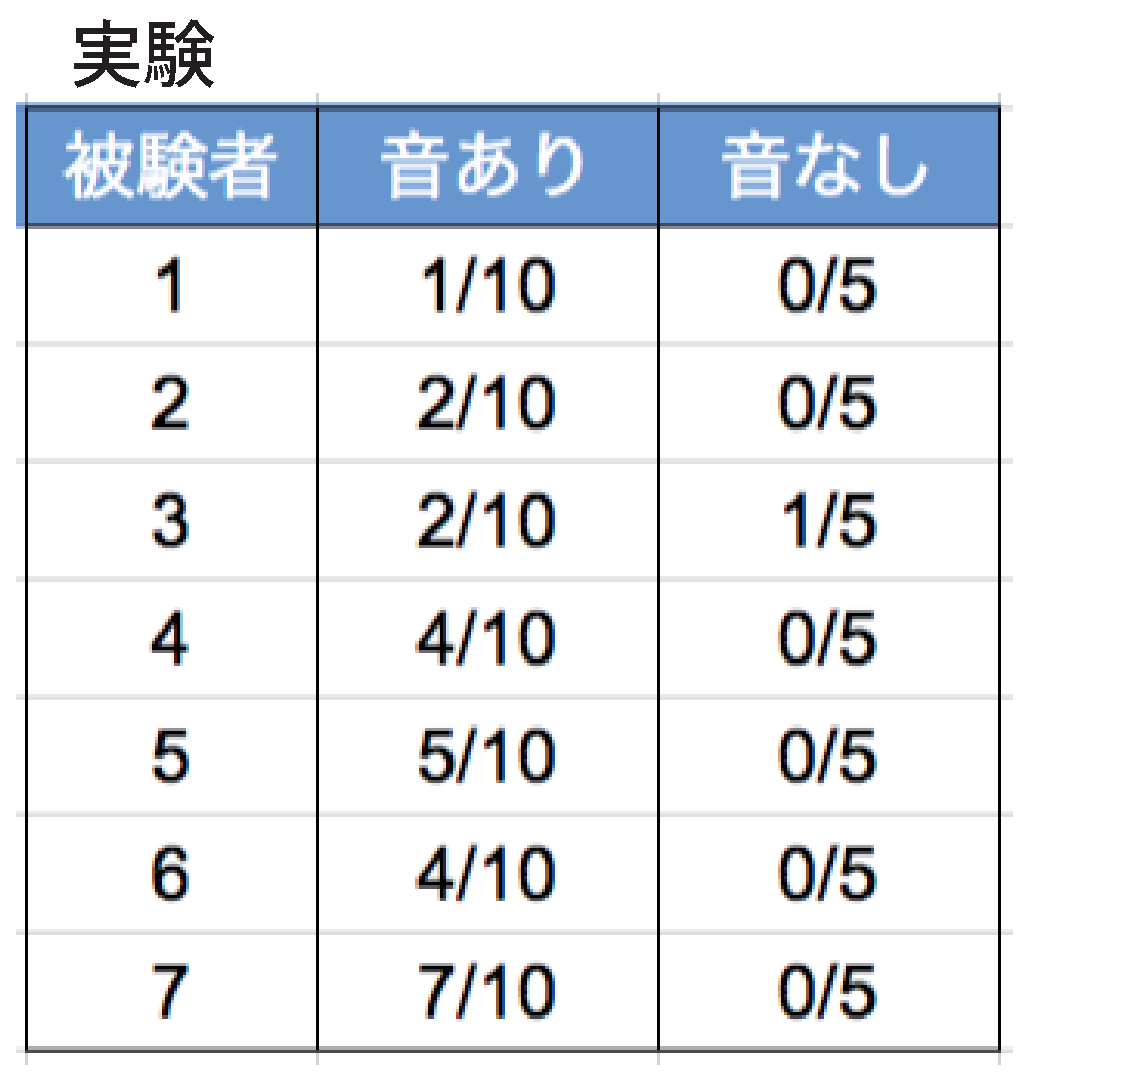
\includegraphics[width=13cm]{eps/musicOnNO.eps}
\caption{音有無の結果}
\label{musciOnNo}
\end{center}
\end{figure}

そこで予備実験を経て浮かび上がった、明晰夢に影響を与える可能性のある要素ごとに実験結果を図\ref{categorizedData}にまとめた。被験者1、被験者2、被験者5、被験者6、被験者7は直接的な体験であるのに対して、被験者3と被験者4は映画を通した間接的な思い出なので間接的と分類した。また思い出から経過している期間も記載した。

\begin{figure}[htbp]
\begin{center}
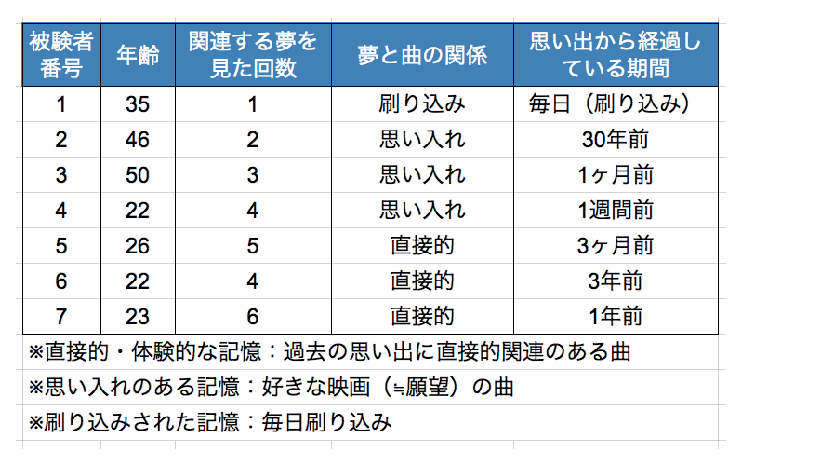
\includegraphics[width=13cm]{eps/categorizedData.eps}
\caption{実験結果のまとめ}
\label{categorizedData}
\end{center}
\end{figure}

図\ref{age}は被験者の年齢と関連する夢を見た回数の相関性を表す図である。直接的な思い出に関連した曲を聴いて寝た被験者は平均的に3.6回夢を見た。比べて間接的な思い出に関連した曲を聴いて寝た被験者は平均的に3.5回夢を見た。加えて予備実験前半に比べて後半の方が夢を見た回数が多いということが図\ref{experiment3}から読み取れる。

\begin{figure}[htbp]
\begin{center}
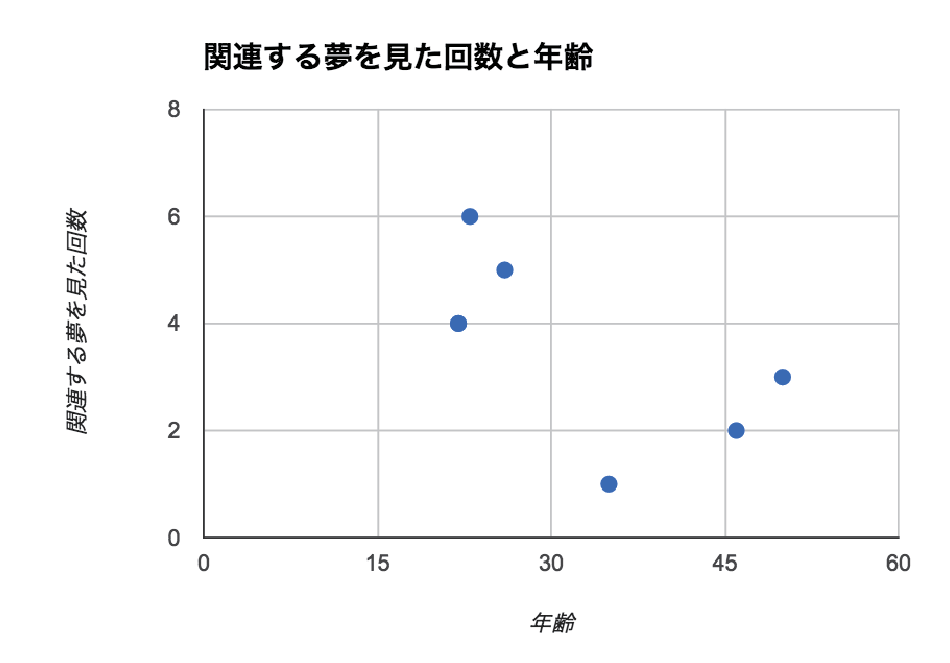
\includegraphics[width=12cm]{eps/age.eps}
\caption{被験者の年齢と関連する夢を見た回数}
\label{age}
\end{center}
\end{figure}

また音の影響によって7人の被験者のうち3人が起きてしまう事態が発生することが分かった。図\ref{result}は音楽を流したタイミング別に結果を表したグラフである。全ての被験者の実験結果を合計しタイミング別に関連した夢を見たときの確率を導き出した。音を流さないときは1/35、レム睡眠中ずっと音を流したときは10/35、そしてレム睡眠中に夢を見たときは13/35の確率で関連する夢を見た。

\begin{figure}[htbp]
\begin{center}
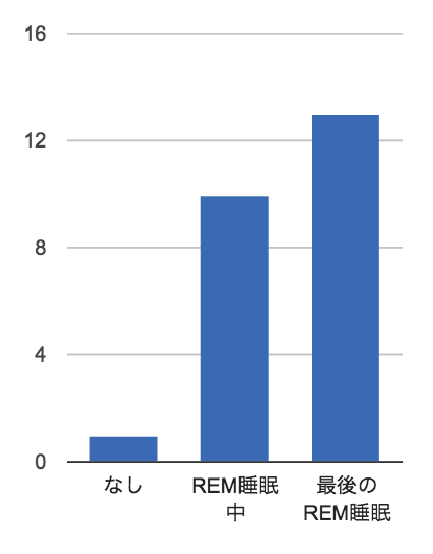
\includegraphics[width=6cm]{eps/result.eps}
\caption{刺激提示のタイミング別の関連した夢を見た回数}
\label{result}
\end{center}
\end{figure}

\section{考察}  
 本論文では研究の目的を
\begin{itemize}
\item 検証1: DreamDateによる明晰夢システムの有効性
\item 検証2: 明晰夢で好ましい仮想体験を味わうことはできるのか
\end{itemize}
と設定したが予備実験と実験結果からこれらについて関連する事象について考察を行う。

\subsection{DreamDateによる明晰夢システムの有効性} 
被験者7人が全員1回以上関連する夢を見ることができた。また予備実験1と本実験の結果から10人中8人が、音で刺激を与えた夜の方が与えなかった夜に対して明晰夢を見る確率が高かった。図\ref{musciOnNo}を参照。この結果はDreamDateの明晰夢システムとしての有効性を示す。

ただ結果には明らかに個人差があった。予備実験から浮かび上がった仮説が
\begin{itemize}
\item 仮説1 : 年齢
\item 仮説2 : その夢を見たいと思う気持ちの強さ
\item 仮説3 : 思い出に関連した曲か否か(どれくらい印象に残っているか・いつの思い出か)
\item 仮説4 : DreamDateの使用期間
\end{itemize}
だったため、それぞれの仮説の検証について述べる。

 実験後「年齢」がDreamDateの効果に影響を与えているか否かに関しては、30歳以下の被験者は平均的に4.75回明晰夢を体験したのに対して、30歳以上の被験者は平均的に2回明晰夢を体験したという結果から、年齢が上がるに連れて明晰夢を体験しにくい体質になる可能性がある。しかし被験者の数が少なすぎて図\ref{age}のグラフからは年齢と結果に相関性を見ることはできなかったため、被験者を増やしてもう一度実験をする必要がある。\\
 実験では「その夢を見たいと思う気持ちの強さ」がDreamDateの効果に影響を与えているか否かに関しては検証できなかった。それはそれぞれの被験者がどのくらいその夢を見たいかを数値的に計ることが難しかったからである。再度実験を行う場合は事前に明晰夢に対する期待度を数値化する必要があるだろう。例えば、「夢をすごく見たい」「夢を見れたら嬉しい」「夢を見れなくてもまぁ仕方ない」のどれかを選んでもらい、実験結果と期待度に壮観がるか否かを検証する必要がある。\\
 「思い出関連した曲か否か」がDreamDateの効果に影響を与えているか否かに関してはある程度検証できた。実験結果によると自ら作曲した歌、演奏した曲、ダンスをした曲などの直接的な記憶にを連想させる音楽を流した被験者5(3ヶ月前にダンスを披露したときの音楽を流した)と被験者6(3年前にバンドで演奏したときの音楽を流した)と被験者7(1年前に作曲した音楽を流した)は10/30の確率で関連性のある夢を見た。次に過去の思い出に関連した音楽を流した被験者1(毎日コーヒーを飲む際の音楽を流した)と被験者2(30年前の結婚式のときの音楽を流した)は3/30の確率で関連性のある夢を見た。一方実際に自分は体験していないが映画などを通して間接的に体験した記憶にまつわる音楽を流した被験者3(1ヶ月前に見た映画の音楽を流した)と被験者4(1週間前に見た映画の音楽を流した)は7/30の確率で夢を見た。図\ref{experiment3}を参照。この結果は流す音がユーザにとって直接的な体験ほど夢に影響を与えやすいということを示唆している。Zhangは夢は記憶の整理をするために見るものだと述べている\cite{Zhang}。被験者Aの場合波の音が過去の記憶を思い出させる音を流すことがトリガーとなり、脳が反応し思い出が夢として再生されたと考えられる。第2章で紹介したDreamOnやユメミールなどのスマートフォンアプリケーションは「鳥の音で森林にいる夢をみることができる」、「貨幣が落ちる音でお金持ちになる夢をみることができる」、「拍手の音で表彰される夢をみることができる」、「フライパンでベーコンが焼ける音で朝食の夢をみることができる」と説明している。しかしユーザはそれぞれ違った経験の持ち主なので全てのユーザにその効果が現れるかの見解には再考の余地が残る。株式会社タカラトミーのホームページでも夢見工房の効果に関しては個人差があると紹介している。その理由もユーザによって音や香りとそれまでの記憶との関連性が違うからだと推測することができる。\\
 「DreamDateの使用期間」については仮設通り、試用期間が長くなるにつれて成功確率が上がったことが図\ref{dates}からわかる。この図はでは図\ref{experiment3}の結果からDreamDateを使用しなかった日数を除いてグラフにした。よって合計10日間の実験と明晰夢を見た被験者の人数の相関図である。被験者の数が少ないので人数を増やしてもう一度実験をする必要がある。
\begin{figure}[htbp]
\begin{center}
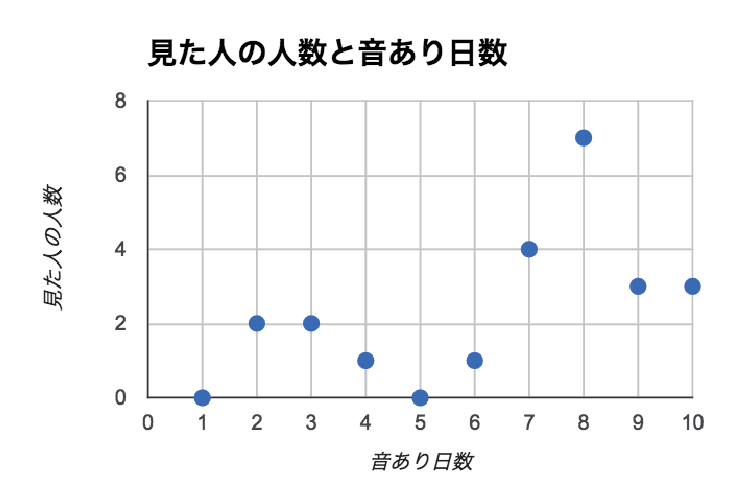
\includegraphics[width=12cm]{eps/experimentDates.eps}
\caption{DreamDateの試用期間と明晰夢を見た回数の相関図}
\label{dates}
\end{center}
\end{figure}

実験を通して明らかにできたことを以下にまとめる。
\begin{itemize}
\item 被験者の思い出とより直接的な音を流すと明晰夢を体験できる確率があがる
\item DreamDateの使用期間が長いほど成功確率が上がる
\end{itemize}

\subsection{DreamDateの有効性を高めるためにできること}
DreamDateには思い出に直結する音を登録する:\\
 本研究を通して、DreamDateで体験できる仮想体験には限界があるということがわかった。人が夢を見るのは過去の記憶を整理するためである。そのためDreamDateでは思い出にない体験や情景を夢で再現することは困難である。実際に予備実験1では海の夢を見た被験者Aと被験者Cはどちらも過去に海に行った際の思い出を夢見たと答えた。一方で海にしばらく行っていない被験者Bは一度も海の夢を見なかった。また予備実験後に行った実験でも、自ら作曲した歌、演奏した曲、ダンスをした曲などの直接的な記憶にを連想させる音楽を流した被験者は10/30の確率、過去の思い出に関連した音楽を流した被験者は3/30の確率で明晰夢を体験したのに対し、自分は体験していないが映画などを通して間接的に体験した記憶にまつわる音楽を流した被験者は7/30の確率でしか夢を見ることができなかった。この結果は被験者の記憶と関連性の高い音を流すと効果が出やすいということが示唆する。よって、明晰夢システムとしてDreamDateで選ぶべき音は思い出に直結する音である。\\

起床時の生活習慣を変える:\\
 全てのユーザが思い出とうまく連携した音を考え付くわけではない。実際に被験者 1 は音楽にあまり関心がなく、特に思い出に残る音・音楽がなかった。そこで最後に行った実験では被験者1に日常生活の中でコーヒーを飲む時に必ず特定の音楽を聴く習慣をつけてもらうことにした。すると図\ref{experiment3}でもあるように実験の最終日でその夢を見ることができた。Ivan Pavlovは条件反射という考え方を提唱している\cite{pavlov}。Pavlovは実験の中で犬に餌を与える前に決まってサイレンを鳴らし続けた結果、サイレンを鳴らすと犬の唾液量が増える現象が起きたと説明している。犬がサイレンを聞くと餌のことを反射的に考えたためだというのが通説である。被験者1は最後の夜に一度夢を見ただけのため、被験者の人数を増やしてさらに精度を上げた実験をする必要があるが、レム睡眠中に音楽が鳴ったことで被験者1に条件反射が働きコーヒーを飲む夢を見た可能性があると考えれる。もし仮説が正しければ、旅行をするときに特定の曲を意識的に繰り返し聴くことで旅行が終わった後もDreamDateでその音を流し旅行での想い出を夢で再生することが可能になる。但し、ある夢を見るために生活のあり方を変えるのは相当高いモチベーションを持ったユーザに限られるだろう。\\

音を流すタイミング:\\
 睡眠中に被験者が起きてしまうと意味がないのだが、ユーザがもっとも起きやすいとされているのはレム睡眠中である\cite{レムノンレム}。そこで予備実験の後に行った実験では被験者を起こさないで明晰夢を促す方法を検証するために音を流すタイミング別に実験結果を検証した。するとレム睡眠中ずっと音を流すのに比べて最期のレム睡眠時にのみ音を流した場合の方が明晰夢を体験できる確率が上がったことが図\ref{result}から読み取れる。この結果からユーザの睡眠が害される可能性を低めるためにタイミングとしては、レム睡眠中ずっとではなく音を流すのは起きる直前のレム睡眠の時が最適であるということが分かった。

\subsection{明晰夢で好ましい仮想体験を味わうことはできるのか} 
DreamDateが提供できる仮想体験の限界:\\
 DreamDateによって全ての被験者が思い出に関連した明晰夢を体験することができた。しかし体験できる夢の内容は限定されている。第2章でオンラインアンケートを行った際に空を飛ぶ夢、サイエンス・フィクションを連想させる夢、アイドルと遊ぶ夢、卒業論文の進め方を教えてくれる夢などそれまでに体験したことのない夢を見たいと答えた人がいたが、そのような夢を見るにはHMDを使った方が適切である。一方でDreamDateで体験可能なのは被験者の思い出に由来した夢である。夢を見ている際、脳は脳が記憶の整理を行っている\cite{Zhang}。DreamDateでは脳の習性を利用して思い出と関連性のある音を流すことで、明晰夢を促す手法をとった。実験では 7人の被験者全員が明晰夢を体験することができた。予備実験2で被験者Cは希望であった遠距離恋愛中の交際相手とデートしたいという要望を実現させることができ、起床後もその体験を忘れずに覚えていた。そして物理的制約を超えて交際相手から手紙が届く夢やデートしている夢を見ることで幸せな気持ちを味わうことができた。DreamDateはVRコンテンツを制作するスキルや時間のないユーザでも気軽に始められるこという利点はあることが証明された。

明晰夢の副作用:\\
 被験者Cは起床後現実は違うということを悟り残念に思う気持ちを味わってしまったとも答えた。明晰夢の副作用についてはDenysがMnemonic Induction of Lucid Dreams (The MILD Technique) で過度に明晰夢を行うと、夢に依存して現実逃避したい気持ちにかられたり睡眠後疲れが取れない現象が起きると説明がある\cite{LaBerge}。よってDreamDateを使うユーザにはあらかじめその現象が起きる可能性があることを了承した上で提供する必要性がある。	% WWW視覚化
\chapter{結論}
\label{chap:coding}
%5.1がまだまだ短すぎ。先輩たちの卒論や修論をまずは読んでみること。実験結果の考察を踏まえて、自分が実現しようとしたことがどの程度実現できてどの程度実現できなかったか、を明確に述べること

本章では本研究の総括を行う。
\section{本研究の総括}
 本研究では明晰夢を実現できる新しい手法として、レム睡眠・ノ ンレム睡眠かを観測し起きる直前のレム睡眠中にユーザが望む体験に関連のある音を流すスマー トフォンアプリケーションDreameDate を開発した。合計15日間7人に使用してもらった結果、全員が1回以上連想する夢を見ることに成功した。Head Mounted Display(HMD)では体験できないようなユニーク且つ現実的(リアルに存在する登場人物や空間)な仮想空間を一部の被験者に提供することができた。また高価なデバイスを購入をせずに既存のスマートフォンにアプリケーションをインストールするだけで使用開始できるツールを構築することができた。\\
 しかし被験者の数が少ないため信ぴょう性の高い実験結果を残すことができなかった。また Mnemonic Induction of Lucid Dreams (The MILD Technique)\cite{LaBerge} に比べて負担のかからないユーザー体験を提供することが目的であったが、結果的に夢日記や寝る前にアプリの起動をしなければならないなどユーザーの負担が増えてしまった。加えて睡眠中夢を見ている時間帯を利用したDreamDateでは体験できる仮想現実のコンテンツに限界があるということがわかった。コンテンツの多様化を目指して音声編集システムの開発や音以外の刺激について検討する必要がある。\\
 一方で実験を通して夢に影響を与えやすい音の種類やタイミングを明らかにすることができた。睡眠時に流す音はユーザー にとって印象に残っている体験に関連している音楽であるほど、高い効果が見込まれる。音声は被験者を起こしてしまうので避けたほうが良い。音を流すタイミングとしては起きる直前のREM睡眠時が良い。こうすることでユーザーの睡眠を害しにくくなり、夢の内容を覚えている確率も高まる。\\
 これまでも音や香りの刺激によって夢を操作する取り組みはされてきた。しかしどのくらいの確率で夢が見れるのかなどの具体的な説明がされている商品はこれまでになかった。よって本解明できた点は必ずしも多くはないが、若干なりとも寄与できたと思われる。

\section{今後の展望}

第4章で述べたが、DreamDateには検討されるべき課題が多い。今後の課題を以下に述べる。

\begin{itemize}
\item より正確且つ大規模な実験\\
本研究での予備実験1,2は筆者自身を含めて家族に協力してもらう結果になった。被験者が家族であると信ぴょう性が低いとみなされるので被験者を再び検討して実験をやり直す必要性がある。また睡眠は被験者の寝ている空間、夢を覚えているか否かの体質、その日の行動や体調が実験の結果に大きく影響を与える。そのため被験者の数をできるだけ多く用意する必要があったのだが、最後の実験でも被験者を7人しか集めることができなかった。当初目的としていた信頼性高いデータを集めるためにも、大規模な実験を行うためにAppStoreにDreamDateを登録することを目指す。\\

\item DreamDate機能面の改善\\
DreamDateは実験用に製作したアプリであるため、App Storeで一般のユーザーに公開するためには機能面での再検討及び改善が望まれる。機能面ではまずユーザー自身が音楽の登録をできるようにする。次に睡眠中、節電のためにディスプレーをOFFにする。DreamDateは一晩中加速度によりモニタリングをする必要がある。現時点ではディスプレーがONになっているので、無駄に電力を消費してしまっている。スマートフォンに備わっている光センサーを利用して、ユーザーがスクリーンを伏せたらディスプレーをシャットダウンさせるシステムにする必要がある。またユーザー体験を向上するために、夢日記機能の手間を減らす必要がある。\\

\item DreamDateユーザー体験の改善\\
現時点ではユーザーは起床後すぐにテキストを入力する仕組みになっているが、音声録音にすることで負担を減らすべきである。また寝る前に他のアプリを使用できない、一晩中充電をしなければならない、睡眠中に音によって起こされてしまうなどの問題を解決してユーザー体験の改善をする必要がある。最後に夢というのはプライベートな情報なので夢日記などのプライバシー強化のための仕組みも必要になるだろう。\\

\item コンテンツの多様化\\
2章の明晰夢で体験したい内容について調査をして、LOVE タイプ、癒しタイプ、元気欲しいタイプ、アドベンチャータイプ、ストーリータイプや、ビジネスタイプなど様々な要望があるのに対して、DreamDateでは特定の音と強く潜在的に思い出のエピソードと結びついている記憶しか夢で再現することができなかった。音声はユーザーを起こしてしまうということで今回は断念せざる得なかったが、音声と音楽をリミックスするなどをして、音声を自動に編集するシステム検討する必要がある。他にも視覚や聴覚の以外にも温度、湿度、振動や体制などによる刺激も試す必要がある。最後に4章でも条件反射の可能性について述べたが、生活の中で特定の行動をするときに音楽を聴く習慣をつけることでどれだけ夢に影響を与えることができるかを実験を通して証明する必要がある。\\

\item 長期的利用が被験者に及ぼす影響を調べる\\
長期的な実験における被験者の生活への影響を考慮するを必要があるだろう。今回は長くて15日間の実験となったが、長期的使用によって睡眠に支障が起きないかを調べる必要がある。睡眠は生物が体を休めるために必要不可欠な行為である。今回DreamDateを使った被験者が睡眠中に起こされてしまったという意見が多数でた。音による睡眠の悪影響について医療の専門家に確認する必要性がある。また明晰夢は経験を重ねるほど、成功率が上がると言われている\cite{LaBerge}。2ヶ月程実験を続けて効果に変化が出るか実験をする必要がある。一方でユーザーが自由自在に夢を操作できるようになった場合、ユーザーがどのような心境になるのかを調べる必要性がある。被験者Cは予備実験を通して夢から覚めて、現実に戻った際に切ない気持ちになってしまった。明晰夢が原因で現実を受け止められれなくなり、結果的にユーザーが悲しむ事態に陥ってしまわないか確かめる必要がある。\\

\item 医療の現場においての有効性を考える\\
本研究の内容が医療の分野で活用されれば、日々失われる記憶の修復ができたり、認知症患者が忘れたくない人や事柄をいつまでも覚えていられるようになる可能性がある。近年ストレスから鬱病や不眠症の悩み抱える社会人が増えているが、DreamDateが夢の中で喜びを与えることで多くの人々を救うことができるかもしれない。\\
\end{itemize}	% 開発手法
\chapter{評価}
\label{chap:ledoxea}
本章では開発したスマートフォンアプリDreamDateの実験方法(調査対象・観察方法)と実験結果について説明する。
	% Androidアプリ「LEDOXEA」
\chapter{結論}
\label{chap:result}

本章では本研究の総括を行う。

\section{本研究の総括}
 睡眠中に外的刺激を与えることで夢の中で拡張現実をのような体験を促すことができるということがわかった。スマートフォンアプリDreamTravelerを使用したで実験で、音をREM睡眠中にユーザーにインプットすることで夢を誘発できるというある程度の成果を出せた。7人の被験者に合計15日間DreamTravelerを睡眠中に使用してもら、最後の7日間に関しては60\%の確率で音に連想する夢をみることに成功した。よって外的刺激により夢をある程度操作することは可能を示している。\\
 実験結果から音に関しては、人の声などを交えるとユーザーが起こされることが分かったので、音声でなく音楽などの方が好ましい。また年齢が若いユーザーの方が比較的夢を操作しやすいということがわかった。私生活が結果に影響をもたらしていることも考えられる。The MILD Techniqueのステップにも含まれている睡眠の前に心を落ち着かせながら特定の夢を見ることを念じる行為や夢日記を書き続ける習慣は明晰夢の確率を上げるのに貢献していることが分かった。睡眠時間が少なく、日々ストレスを感じている被験者は音の有無関係なく会社での仕事の夢を見る。日常的に音楽を聞かないユーザーに対しても効果が得られた。具体的にはコーヒーを飲むたびに同じ音楽を聴いてもらった。すると、睡眠中にその音楽を流したときにコーヒーの夢を見ることができたのである。\\
 他の研究でも、音や香りの刺激によって夢を操作する取り組みはされてきた。しかしどのくらいの確率で夢が見れるのか、どのような音楽が適しているのかなどの具体的な説明がされている商品はこれまでになかった。よって本解明できた点は必ずしも多くはないが、若干なりとも寄与できたと思われる。
 DreamTravelerによってユーザは思い出を夢で再生することができるようになり、物理的に会うことのできない人と会話をしたり、過去の思い出でもう一度過ごすことで睡眠をより楽しむことができるなどこれまでにない新しい睡眠のスタイルの実現となる。

\section{今後の展望}
今回の解決すべき命題は、
\begin{itemize}
\item アプリの製作:\\
実験において被験者から自分たちで音楽の登録ができるようにしたいという意見が出た。ここからDreamtravelerの機能面での再検討及び改善が望まれる。

\item 音による睡眠の悪影響についてえ医療の専門家に確認:\\
睡眠中に起こされてしまったという意見がでた。音による睡眠の悪影響について医療の専門家に確認する必要性がある。

\item 思い出の多様化:\\
2章の明晰夢で体験したい内容について調査したが、実際DreamTravelerでは特定の音と強く潜在的に思い出のエピソードと結びついている記憶しか夢の中で再生することができなかった。本研究では視覚や聴覚の刺激しか実験しなかったが、睡眠は他にも数多くの刺激と関係性がある。温度、湿度、振動や、体制などによる刺激も考える必要がある。

\item より大人数の実験を行う\\
音楽を流すタイミング、期間、音の種類をについてより細かい実験を行いたい。そのためにもアプリをいち早くAppStoreに登録することでより多くの人たちに使ってもらうことを目指す。

\item 医療の現場においての有効性を考える\\
本研究の分野が多岐にわたって進めば日々失われる記憶の修復ができたり、忘れたくない人をいつまでも覚えていられるようになる可能性がある。認知症や鬱病を抱えている患者に喜びを与えられたり、悪夢に悩まされている人々を救うことができるかもしれない。

\end{itemize}

の4点であった。	% アンケートによる評価と考察
%\chapter{結論}
\label{chap:conclusion}
本研究では睡眠中に思い出に関連した音を流すことでその音に関連した夢を見ることを促進するシステム、DreamScapeを提案、施策した。明晰夢をスマートフォンアプリによって誘発するためのある程度の成果と、今後の課題や方針を得られたと考える。それらを以下に示す。

\section{本研究の総括}
DreamScapeによってユーザは思い出を夢で再生することができるようになり、拡張現実を体験できるようになれば、物理的に会うことのできない人と会話をしたり、過去の思い出でもう一度過ごすことで睡眠をより楽しむことができるなど、これまでにない新しい睡眠のスタイルの実現となる。
 拡張現実や睡眠に関する調査から睡眠中の夢をコントロールすることにはニーズは充分あると確信し、より多くの人たちが簡単にアクセスできるようにスマートフォンアプリ、DreamScapeを開発をした。携帯に備わっている加速度センサーでREM睡眠(夢を見ているタイミング)を観測し、そのタイミングでユーザー記憶を思い出させる音を流し、ユーザーの夢を刺激、誘導すことを目的としたシステムである。
 4人の被験者に合計20日間DreamScapeを睡眠中に使用してもらった結果、最後の7日間に関しては65\%の確率で音に連想する夢をみることに成功した。明晰夢を実現するために効果的な音楽の種類や音楽を流すタイミングなどを知ることができた。またDreamScapeの導入により、睡眠がより楽しいものになると見込まれた。

\section{今後の展開}

\subsection{再度アプリの製作}
実験において、被験者からもっと簡単に音楽の登録をできるようにしたいという意見が出た。ここからDreamScapeの機能面での再検討及び改善が望まれる。また、睡眠中に起こされてしまったという意見がでた。音による睡眠の悪影響について医療の専門家に確認する必要性がある。

\subsection{実験の精度をあげて大人数での実験を行う}
実験の精度をあげて音楽を流すタイミング、期間、音の種類をについてより細かい実験結を行う。そのためにもアプリをAppStoreに登録することでより多くの人たちに使ってもらう。

\subsection{夢を見るために現実を加工することも検討}
DreamScapeの最大の難点は思い出に関連する音楽を見つけなければならないことだ。人によっては音楽をあまり聞かない人もいる。そこで生活のあり方を変えてみるのだ。例えばコーヒーを飲む時に必ず特定の音楽を聞くことで、その音楽を流すことで夢が操作される可能性が高まる。しかし生活がDreamScapeを使用することで変容していくと予想されるため、それが人によって良い影響であるのかの検討も必要である。

\subsection{医療の現場でにおいての有効性を考える}
本研究の分野が多岐にわたって進めば日々失われる記憶の修復ができたり、忘れたくない人をいつまでも覚えていられるようになる可能性がある。認知症や鬱病を抱えている患者に喜びを与えられたり、悪夢に悩まされている人々を救うことができる。


%\begin{itemize}
%\item Mashupによって、e-learningコンテンツを素早く、便利に検索するための手法を提案できた。
%\item 納豆ビューを参考として、よりスマートフォン端末に最適化した形でのグラフ型WWW視覚化を発案できた。
%\item Android端末上であることを意識し、ユーザにとって容易な操作方法を実装した。
%\end{itemize}

%\section{今後の課題と方針}
%\begin{itemize}
%\item 別のプラットフォームに対しての移植が可能であるかどうかを検討し、デバイス毎にチューニングを施していくことを考える。
%\item それぞれの検索結果をより深く融合して、特徴空間におけるコンテンツの特徴ベクトルに基づくシステムへ再構成し、よりシンプルに結果まで辿り着くようにする。
%\item ユーザが、より思ったとおりの操作を実現できるよう、メソッドや操作方法を追加・編集し、アプリとしてのユーザビリティを向上させる。
%\item 画像ファイルの扱いをより極小化し、応答速度の向上を目指す。
%\item 現在残っている数種のバグを取り除き、アプリとしての完成度をより高める。
%\end{itemize}	% まとめ


%//実験に参加してもらった人の名前を列挙しても良いと思う

\begin{acknowledgment}
本研究を進めるにあたり、絶えず懇切丁寧なご指導を頂きました、慶應義塾環境情報学部中西泰人教授に深く感謝いたします。 また使用実験にAnditto Heristyoさん、Josh Eitenさん、Daniel Kimさん、樋山幸治さん、樋山幸子さん、樋山さとみさん、Brian Hayashiさんにご協力いただきました。ここに深い感謝の念を表します。 最後に、慶應義塾大学中西研究室学部生の皆様に深く感謝し、謝辞といたします。 
\end{acknowledgment}
	% 謝辞。要独自コマンド、include先参照のこと
\begin{bib}[100]


% \bibitem{参照用名称}
%   著者名: 
%   \newblock 文献名,
%   \newblock 書誌情報,出版年.

\bibitem{vrtrendShiny}
\begin{flushleft}
  Shiny Mathew:
  \newblock Importance of Virtual Reality in Current World,
  \newblock International Journal of Computer Science and Mobile Computing A Monthly Journal of Computer Science and Information Technology IJCSMC, Vol. 3, Issue. 3, 3, March 2014, pg.894 \UTF{2013} 899,
\end{flushleft}

\bibitem{vrtrendSamuel}
\begin{flushleft}
  Samuel Ebersole:
  \newblock A Brief History of Virtual Reality and its Social Applications, Academia.edu,
  \newblock Jan 1, 1997,  pg.3.
\end{flushleft}

\bibitem{dream}
\begin{flushleft}
『大辞泉 第二版』小学館:
  \newblock 2012 年 11 月 2 日
 \end{flushleft}

\bibitem{saintDenys}
\begin{flushleft}
Hervey de Saint-Denys:
  \newblock Transl.: Dream and the Ways to Direct Them: Practical Observations
  \newblock 1867
  \newblock Paris: Librairie d'Amyot, \UTF{00C9}diteur, 8, Rue de la Paix.
 \end{flushleft}
 
 \bibitem{saintDenys}
\begin{flushleft}
Hervey de Saint-Denys:
  \newblock Dream and the Ways to Direct Them: Practical Observations
  \newblock 1867
  \newblock Paris: Librairie d'Amyot, \UTF{00C9}diteur, 8, Rue de la Paix.
 \end{flushleft}
 
  \bibitem{LaBerge}
\begin{flushleft}
 LaBerge Stephen and Howard Rheingold:
  \newblock Exploring the World of Lucid Dreaming
  \newblock New York: Ballantine, 1990. Print.
 \end{flushleft}
  
\bibitem{takaratomi}
\begin{flushleft}
  タカラトミー:
  \newblock "好きな夢が見られる? タカラの安眠グッズ「夢見工房」." ,
  \newblock ITmedia LifeStyle. N.p., n.d.
  \newblock Web. 08 Jan. 2016.
  \newblock{\it http://www.itmedia.co.jp/lifestyle/articles/0401/14/news047.html}.
\end{flushleft}

\bibitem{dreamOn}
\begin{flushleft}
  Dream:ON:
  \newblock "Dream:ON - The App to Influence Your Dreams.",
  \newblock The App to Influence Your Dreams. N.p., n.d. Web.
  \newblock Web. 08 Jan. 2016.
  \newblock{\it http://www.dreamonapp.com/}.
\end{flushleft}

\bibitem{freud}
\begin{flushleft}
  Sigmund Freud:
  \newblock The Interpretation of Dreams (1900).,
  \newblock Sigmund Freud: The Interpretation of Dreams</i>. N.p., n.d. 2015.
\end{flushleft}

\bibitem{beddit}
\begin{flushleft}
  beddit.com:
  \newblock Beddit Sleep Monitor and the Science Behind It,
  \newblock Beddit Science Leafle HR, 29 Aug. 2014.
\end{flushleft}

\bibitem{neuroon}
\begin{flushleft}
  Neuroon:
  \newblock  "Neuroon - an Intelligent Sleep Mask."
  \newblock Neuroon. N.p., n.d. Web. 08 Jan. 2016.
  \newblock{\it https://neuroon.com/technology/}.
\end{flushleft}

\bibitem{beWellApp}
\begin{flushleft}
  Zhenyu Chen, Mu Lin, Fanglin Chen, Nicholas D. Lane, Giuseppe Cardone, Rui Wang, Tianxing Li, Yiqiang Chen, Tanzeem Choudhury, Andrew T. Campbell:
  \newblock  Unobtrusive Sleep Monitoring using Smartphones,
  \newblock 2013 7th International Conference on Pervasive Computing Technologies for Healthcare and Workshops, pg. 145~152,
  \newblock 2013.252148
\end{flushleft}

\bibitem{iSleep}
\begin{flushleft}
  Tian Hao, Guoliang Xing, Gang Zhou:
  \newblock  iSleep: Unobtrusive Sleep Quality Monitoring using Smartphones,
  \newblock SenSys’13,
  \newblock  November 11\UTF{2013}15, 2013, Rome, Italy
\end{flushleft}

\bibitem{sleepSheep}
\begin{flushleft}
  長塚 麻美, 串山 久美子, 馬場 哲晃:
  \newblock  The Interface to Improve the Quality of Sleep by the Sleep Depth Determination Using the Motion Detection,
  \newblock 情報処理学会 インタラクション 2015 IPSJ Interaction 2015,
  \newblock  A16 2015/3/5,
\end{flushleft}

\bibitem{iWinks}
\begin{flushleft}
iWinks:
 \newblock  "The Ultimate Lucid Dreaming Tool." ,
  \newblock N.p., n.d. Web. 08 Jan. 2016,
  \newblock{\it https://iwinks.org/}.
\end{flushleft}

\end{bib}	% 参考文献。要独自コマンド、include先参照のこと
\appendix
\chapter{プログラム}
実装したアプリのソースコードを掲載する。実装はswift7.0を用いて、iPhone 9.2での動作を確認している。またこのプログラムのパブリッシュ、デバッグのためには以下のライブラリ、フレームワーク、画像ファイルが必要となるため、導入・設定の後実行する必要がある。
\begin{itemize}
\item Away3D 4.1.0 Alpha (away3d-core-fp11\_4\_1\_0\_Alpha.swc)\cite{away3d}
\item Bulk Loader (bulk\_loader.swc)\cite{bulkloader}
\item As3 Crypto (as3crypto.swc)\cite{as3crypto}
\item norm-top.png (128x128px のpngファイル)
\item norm.png (128x128px のpngファイル)
\item img-top.png (128x128px のpngファイル)
\item img.png (128x128px のpngファイル)
\item doc-top.png (128x128px のpngファイル)
\item doc.png (128x128px のpngファイル)
\item mv-top.png (128x128px のpngファイル)
\item ama-top.png (128x128px のpngファイル)
\item ama.png (128x128px のpngファイル)
\item defImgXML.xml (Y!画像検索APIにて取得したダミー用のXMLファイル)
\end{itemize}

これらソースコードパッケージの最新版はGithubの以下のURLにて公開している。 

https://github.com/legnoh/ledoxea
		% 付録

\end{document}
